%                                                                 aa.dem
% AA vers. 9.1, LaTeX class for Astronomy & Astrophysics
% demonstration file
%                                                       (c) EDP Sciences
%-----------------------------------------------------------------------
%
%\documentclass[referee]{aa} % for a referee version
%\documentclass[onecolumn]{aa} % for a paper on 1 column  
%\documentclass[longauth]{aa} % for the long lists of affiliations 
%\documentclass[letter]{aa} % for the letters 
%\documentclass[bibyear]{aa} % if the references are not structured 
%                              according to the author-year natbib style

%
\documentclass{aa}  

%
\usepackage{graphicx}
%%%%%%%%%%%%%%%%%%%%%%%%%%%%%%%%%%%%%%%%
\usepackage{txfonts}
%%%%%%%%%%%%%%%%%%%%%%%%%%%%%%%%%%%%%%%%
%\usepackage[options]{hyperref}
% To add links in your PDF file, use the package "hyperref"
% with options according to your LaTeX or PDFLaTeX drivers.
%
\begin{document} 


   \title{The variability  of Betelgeuse explained by surface convection\thanks{Based on observations obtained at the T\'elescope Bernard Lyot
   (TBL) at Observatoire du Pic du Midi, CNRS/INSU and Universit\'e de
   Toulouse, France.}}
 

    \author{{ Q.~Pilate}\inst{1},{ A.~L{\'o}pez Ariste}\inst{1},{ A.~Lavail}\inst{1},{ Ph. Mathias}\inst{1} }

   \institute{IRAP, Universit\'e de Toulouse, CNRS, CNES, UPS.  14, Av. E. Belin. 31400 Toulouse, France 
             }

   \date{Received ...; accepted ...}

% \abstract{}{}{}{}{} 
% 5 {} token are mandatory
 
  \abstract
 

   \keywords{
               }

   \maketitle
%
%-------------------------------------------------------------------

\section{Introduction}
\label{sec:introduction}
Betelgeuse is a prototypical red supergiant (RSG), known to be a semi-regular variable. Several periods can be found in the 
literature, usually clustered around the so-called long secondary period (LSP) of 2000 d, plus shorter periods around 400 and 200 d \citep{kiss_variability_2006}. The origin of the LSP remains a source of discussion: some have tried to find the explanation of the LSP in the lifetime of the large convective cells present at the surface of RSGs \citep[e.g][]{stothers_giant_2010} while others have invoked a magnetic field \citep{wood_long_2004}. The shorter periods of 400 and 200 d are given a different origin than the LSP. By studying a large sample of RSGs, \cite{kiss_variability_2006} attributed the 400 d period to radial pulsation modes, while the 200 d period being attributed to the first overtone \citep{joyce_standing_2020}, in agreement with the historical work of \cite{stothers_pulsation_1969}.\\

Besides radial pulsation, surface activity leading to random brightness variations has also been mentioned to explain the variability of Betelgeuse, first theorised by \cite{schwarzschild_scale_1975}. More recently, \cite{gray_mass_2008} proposed that the 400 d period was a consequence of convective activity. Betelgeuse is known to present large convective cells with lifetimes of the order of one to two years \citep{lopez_ariste_convective_2018} and measurable changes 
within the span of one week. Bright convection cells near the disk center will increase the integrated brightness of the star compared with other situations where such cells are found near the edges. So, even without invoking the formation of 
dust or other changes in opacity, one may argue that the simple evolution of convective patterns of the star may create variability. Such 
variability could be expected to be random, but will present quasi-periodicities related to the typical time scales of the 
convective patterns \citep{gray_mass_2008}. \\

%more or less well defined 
%periods around 400 and 200 days. 
%Such periods are often linked to radial pulsation modes,   and have been used to model 
%the characteristics of the resonant cavity, hence the size of the star and eventually its evolutionary stage \citep{saio_evolutionary_2023}.


At the end of 2019, Betelgeuse reached a historical minimum in its luminosity, called the Great Dimming \citep{guinan_fall_2020}. 
From interferometric and spectroscopic data, it has been proposed that this event was caused by the formation of a cloud of dust close to the line of sight \citep{montarges_dusty_2021}. 
Interferometric images show a drop in luminosity in the southern hemisphere of Betelgeuse, which could be caused by a mass loss event and leading to this dimming \citep{dupree_great_2022}. Other hypotheses have also been explored, such as a drop in temperature \citep{harper_photospheric_2020}, or an increase in the molecular opacity \citep{kravchenko_atmosphere_2021}. 
In this event, it turns out that a change in brightness was not  due to pulsation but to a change in the 
brightness distribution over the stellar disk.
%due to the presence of large quantities of dust.
Since the end of the Great Dimming event, Betelgeuse has continue its random variation of brightness. 
But quite interestingly, 
it has been shown by \cite{jadlovsky_analysis_2023} and \cite{dupree_great_2022} that the periodicity of Betelgeuse has changed since the dimming. Using the light curves from AAVSO, 
the cited authors showed that before the dimming, the dominant period of Betelgeuse was the 400 d period, while after the great dimming, the main periods of Betelgeuse have shortened, oscillating between 97 d and 230 d \citep{dupree_great_2022}, revealing a change in the behaviour of the atmosphere of Betelgeuse.
While the great dimming may be seen as 
a singular event, such modifications of the variability periods bring up the question of whether all changes in brightness can be due to similar changes in the brightness 
distribution over the disk and unrelated to any pulsation phenomenon. 
Our interest in an alternative explanation of the variability
in terms  of convective patterns arose. In order to address this question, we seek such typical periods of 400 and 200 d in  
observational proxies related to the convective
activity but not to any pulsation, such as the linear polarization
spectra.\\
%but unrelated to pulsations and which cannot be directly linked to brightness.
%Faced with the dramatic change in stellar parameters and age that such change in a pulsation period would 
%require, 

Linear polarization in the atomic lines of the spectrum of Betelgeuse, discovered by \cite{auriere_discovery_2016}, has been interpreted as the joint action of 
two mechanisms. First, the depolarization of the continuum by atoms which absorb linearly polarized light from the continuum and re-emit unpolarized light,
the continuum photons being polarized by Rayleigh scattering. This depolarization produces signals with azimuthal symmetry over the visible disk, which would  cancel out the net linear polarization on a homogeneous disk. Thus, such mechanism of polarization must be combined with an inhomogeneous disk to produce the net linear polarization 
signal observed. This interpretation suggested the possibility of mapping those brightness inhomogeneities. This has been achieved by \cite{lopez_ariste_convective_2018}, who produced even 3-dimensional images of the atmosphere of Betelgeuse \citep{lopez_ariste_three-dimensional_2022} by taking advantage of the different heights of formation of 
different lines in the spectrum of Betelgeuse. The produced images compare very well with contemporaneous images made with interferometric 
techniques \citep{montarges_close_2016} and show clear convective patterns, akin to solar granulation.\

Linear polarization observed in the atomic lines is therefore a proxy of convection, a priori unrelated to radial 
pulsations but linked to the brightness inhomogeneities due to the convective patterns in Betelgeuse. If one can find the aforementioned variability periods 
in linear polarization, we must conclude that these periods are related to the convective activity which originates the linear polarization signals.
%and unrelated to any radial pulsation phenomena. 
This is the purpose of the present work.\

In section \ref{Section 2}, we describe the dataset of linear polarization obtained with Narval and Neo-Narval at the 2-metre T\'elescope Bernard Lyot (TBL), as well as the Lomb-Scargle periodograms used to derive periods. In section \ref{section 3}, we seek periods in the LSD profiles of Betelgeuse using the Lomb-Scarlge periodogram. In section \ref{section 4}, we associate the 200 d period with the convective timescale of the smallest granules and the 330 d periodicity with the largest granules. We speculate on an explanation in the change of variability of Betelgeuse before and after the great dimming. 


\section{The polarimetric data}
\label{Section 2}

Betelgeuse has been observed for the last 10 years with Narval and Neo-Narval at the Telescope Bernard Lyot\footnote[1]{https://tbl.omp.eu/}. These two instruments measure the polarization 
over the visible and near infrared spectra of Betelgeuese (390-1000 nm) with high spectral resolution (R=65000) and high polarimetric sensitivity. The signal-to-noise ratios are not sufficient to measure the weak polarization signals in individual atomic lines of the 
spectrum. These amplitudes are known to be of the order of $10^{-4}$ times the continuum intensity, and they only exceptionally reach amplitudes of $10^{-3}$. When these high amplitudes are present, enough photons can be accumulated per spectral bin to 
detect the linear polarization signal above noise in lines \citep{auriere_discovery_2016}. Most commonly, the amplitudes of linear polarization are below noise levels. On those 
occasions, we have to add up the signals of thousands of lines to increase the signal-to-noise ratios. This addition 
is performed through the Least-Squares Deconvolution technique \citep[LSD;][]{donati_spectropolarimetric_1997,2010A&A...524A...5K}.% and assumes that the 
%linear polarization signal is similar 
%in all spectral lines up to scale factors in the sampling and amplitude.
This technique has been successfully used in the past to measure 
magnetic field distributions over stellar surfaces \citep[e.g][]{donatiLandstreet2009,reiners2012,kochukhov2021} and is now employed to produce images of the brightness distributions in the photosphere 
of Betelgeuse and other RSGs, as cited in section~\ref{sec:introduction}. 

In this work, we shall examine the signals produced through the LSD technique, which produce a pseudo-spectral line in intensity 
and linear polarization. This pseudo-spectral line does not correspond to any particular atomic species but rather represents an average of all species present and emitting in the 
photosphere of Betelgeuse. Following these procedures of line addition, the resulting profiles carry the coherent signals present in the photospheric lines, but the specific characteristics of individual spectral lines are erased. All of this data has been previously presented before by \cite{auriere_discovery_2016}, \cite{mathias_evolution_2018} and 
\cite{lopez_ariste_three-dimensional_2022}, which also provide details on observing times and conditions as well as a more detailed description 
of the data reduction process\footnote[2]{Beyond a 2-year proprietary embargo, and up to technical issues, all these data is available through 
PolarBase (http://polarbase.irap.omp.eu/).}.\\
Note that all the velocities mentioned in the text or in the figures are provided in the heliocentric frame.



%\subsection{Lomb-Scargle periodograms of the profiles}

\section{Period search}
\label{section 3}


Attempting to identify periods in an astrophysical context faces the challenge of unevenly spaced observed data. To overcome this hurdle, 
we used the Lomb-Scargle periodogram \citep{lomb_least-squares_1976,scargle_studies_1982}. This method involves fitting sinusoids to the data using least-squares with frequency sampled between the first and last observation. The quality of the fit determines the power attributed to a frequency. We applied this technique to the  LSD profiles of Stokes $I$, $U$, $Q$ and to the total linear polarization of Betelgeuse observed by the TBL over a span of 10 years (2014-2024). However, the dataset available post-dimming is insufficient to produce meaningful periodograms. Therefore, our focus was on periodograns computed exclusively from data obtained before the great dimming, covering the period from 2014 to the end of 2019. 

\subsection{Variability of the Stokes parameters}

We first computed the Lomb-Scargle periodogram at each wavelength of the LSD profile, ranging from -25 km/s to +60 km/s to cover the entire 
signal present in the LSD profile. \cite{lopez_ariste_convective_2018} identified the most blueshifted signal towards -20 km/s and interpreted it as  the maximum velocity of the rising plasma. The most redshifted signal was often found at +40 km/s, interpreted 
as the rest velocity of the star. Sometimes, signals at velocities greater than +40 km/s can be found, which can be interpreted either as dark and cold plasma falling back to Betelgeuse or as rising plumes of plasma located on the hidden face of Betelgeuse, ascending so high that they appear above the limb \citep[for the case of the RSG $\mu$~Cep]{lopez_ariste_height_2023}.





% The LS periodogram  computed for each frequency 
% in the LSD profile must show periodicities around the LSP, but also on the 400 days and 200 days period. If the LS periodogram finds a periodicity at a
% given wavelength, it would appear as a strong LS power. However, we expect a change in the periodicity after the dimming. 
% This would lead to a decrease in the Lomb-Scargle power. By comparing LS periodogram before and after the dimming, we expect to see a change in the LS power,
% especially at the 400 days period. 

Figures \ref{LS intensity},\ref{LS Q},\ref{LS U} and \ref{LS linear polarization} show the Lomb-Scargle periodogram of the LSD profile for Stokes $I$, Stokes $Q$, Stokes $U$ and the total linear polarization, respectively. 
%The abscissa is the frequency (in $\mathrm{days^{-1}}$), while the ordinate is the heliocentric radial velocity in km/s. 
In each figure, the upper panel depicts the Lomb-Scargle periodogram of each velocity bin (grey lines) along with the total average (red line). The green line represents the window function. The lower panel shows the Lomb-Scargle periodogram for each velocity bin, with the white dotted lines marking the 400 and 200 d periods for reference. The right panel represents the mean profile of each Stokes parameter at each velocity bin.

\begin{figure}[!h]
    \centering
    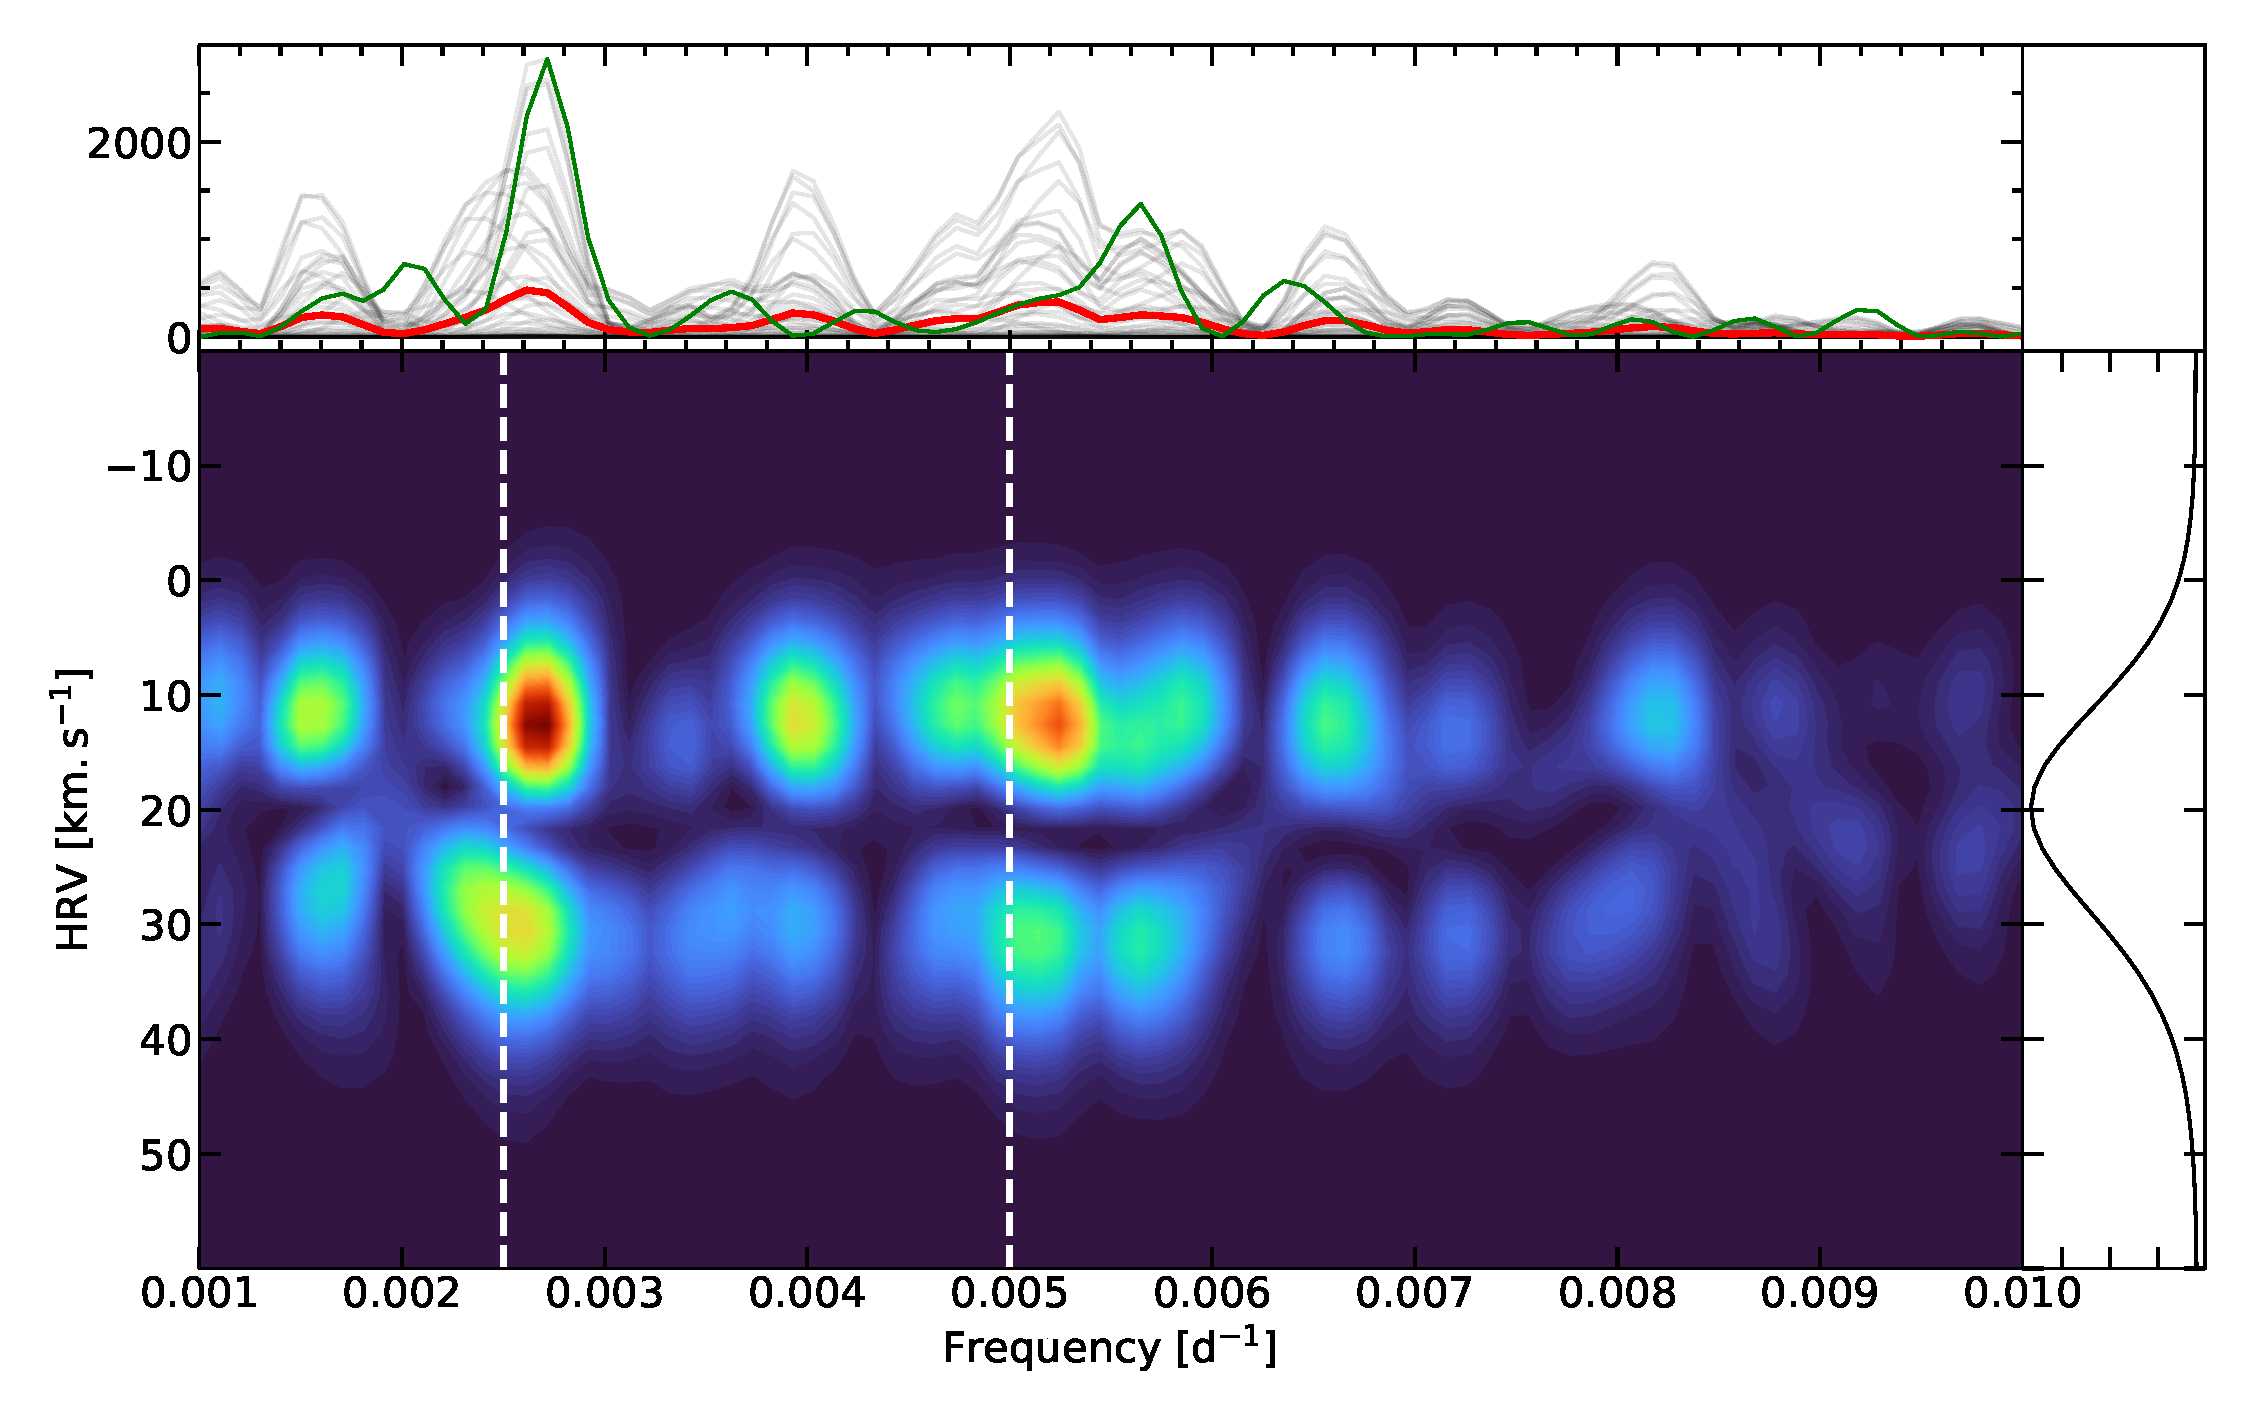
\includegraphics[width=0.5\textwidth]{Lomb-Scargle Intensity.pdf}
    \caption{Lomb-Scargle periodogram of the LSD profile of intensity.
    The upper panel is the Lomb-Scargle periodogram for each velocity bin (grey lines) and the average (red line). The green line is the window function.
    In the lower panel, the two white dashed lines mark respectively the 400 d and the 200 d periods. The right panel is the average intensity profile for each velocity bin.}
    \label{LS intensity}
\end{figure}

\begin{figure}[!h]
    \centering
    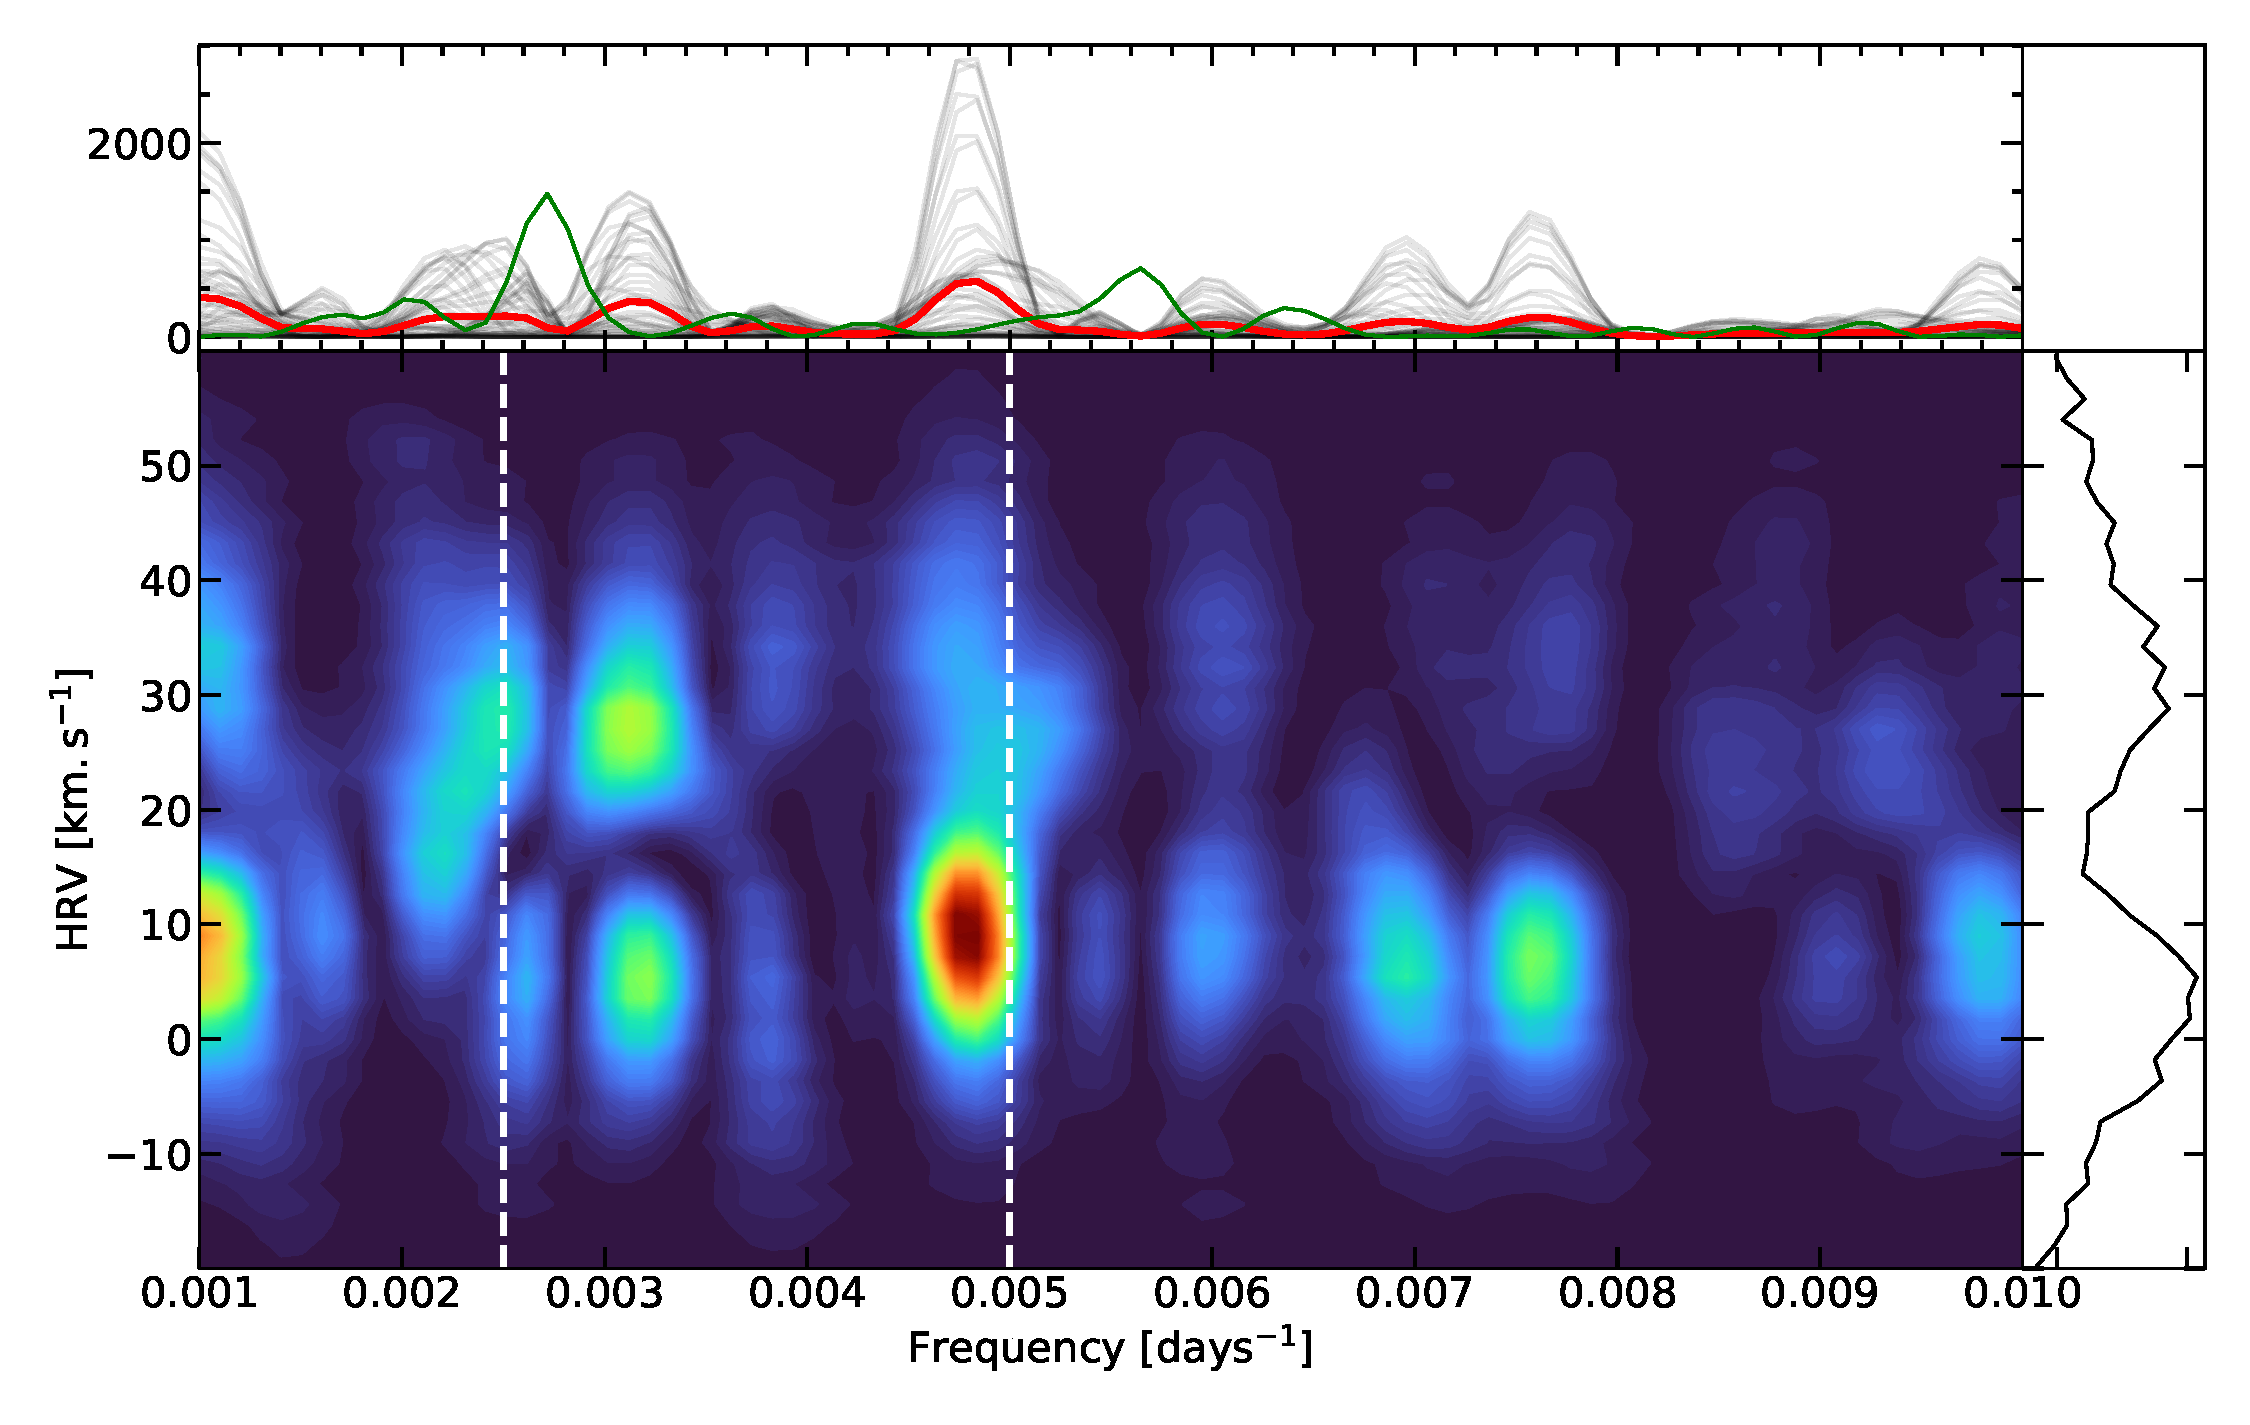
\includegraphics[width=0.5\textwidth]{Lomb-Scargle Stokes Q.pdf}
    \caption{Same as Fig. \ref{LS intensity} for Stokes $Q$. }
    \label{LS Q}
\end{figure}

\begin{figure}[!h]
    \centering
    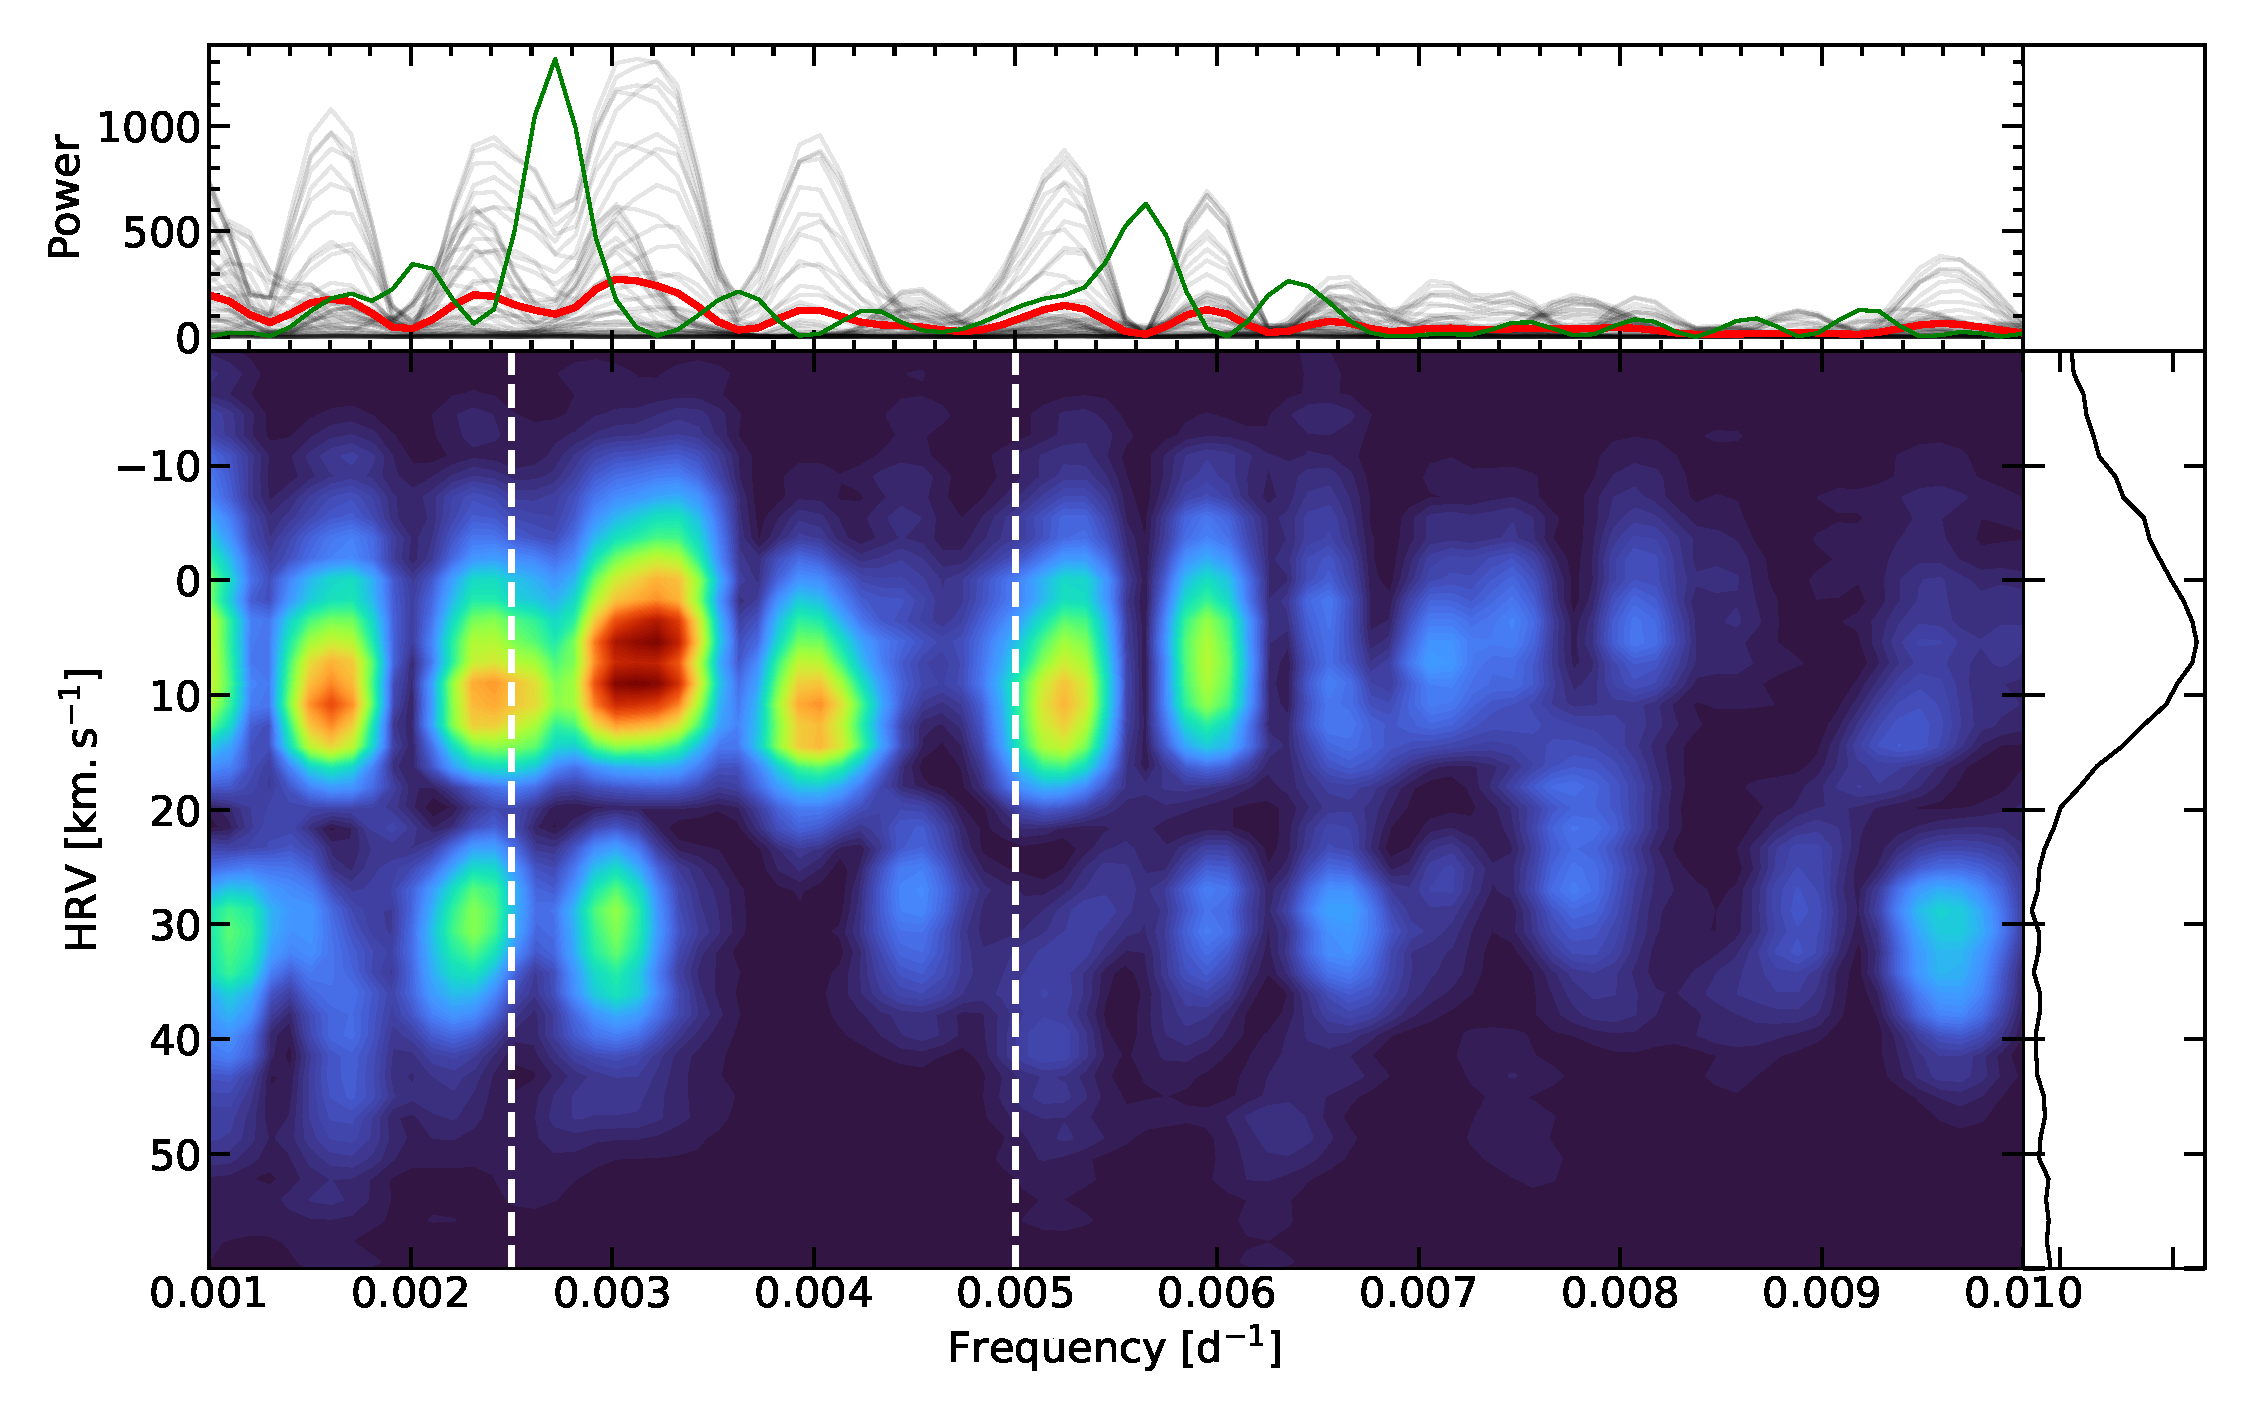
\includegraphics[width=0.5\textwidth]{Lomb-Scargle Stokes U.pdf}
    \caption{Same as Fig. \ref{LS intensity} for Stokes $U$.}
    \label{LS U}
\end{figure}


\begin{figure}[!h]
    \centering
    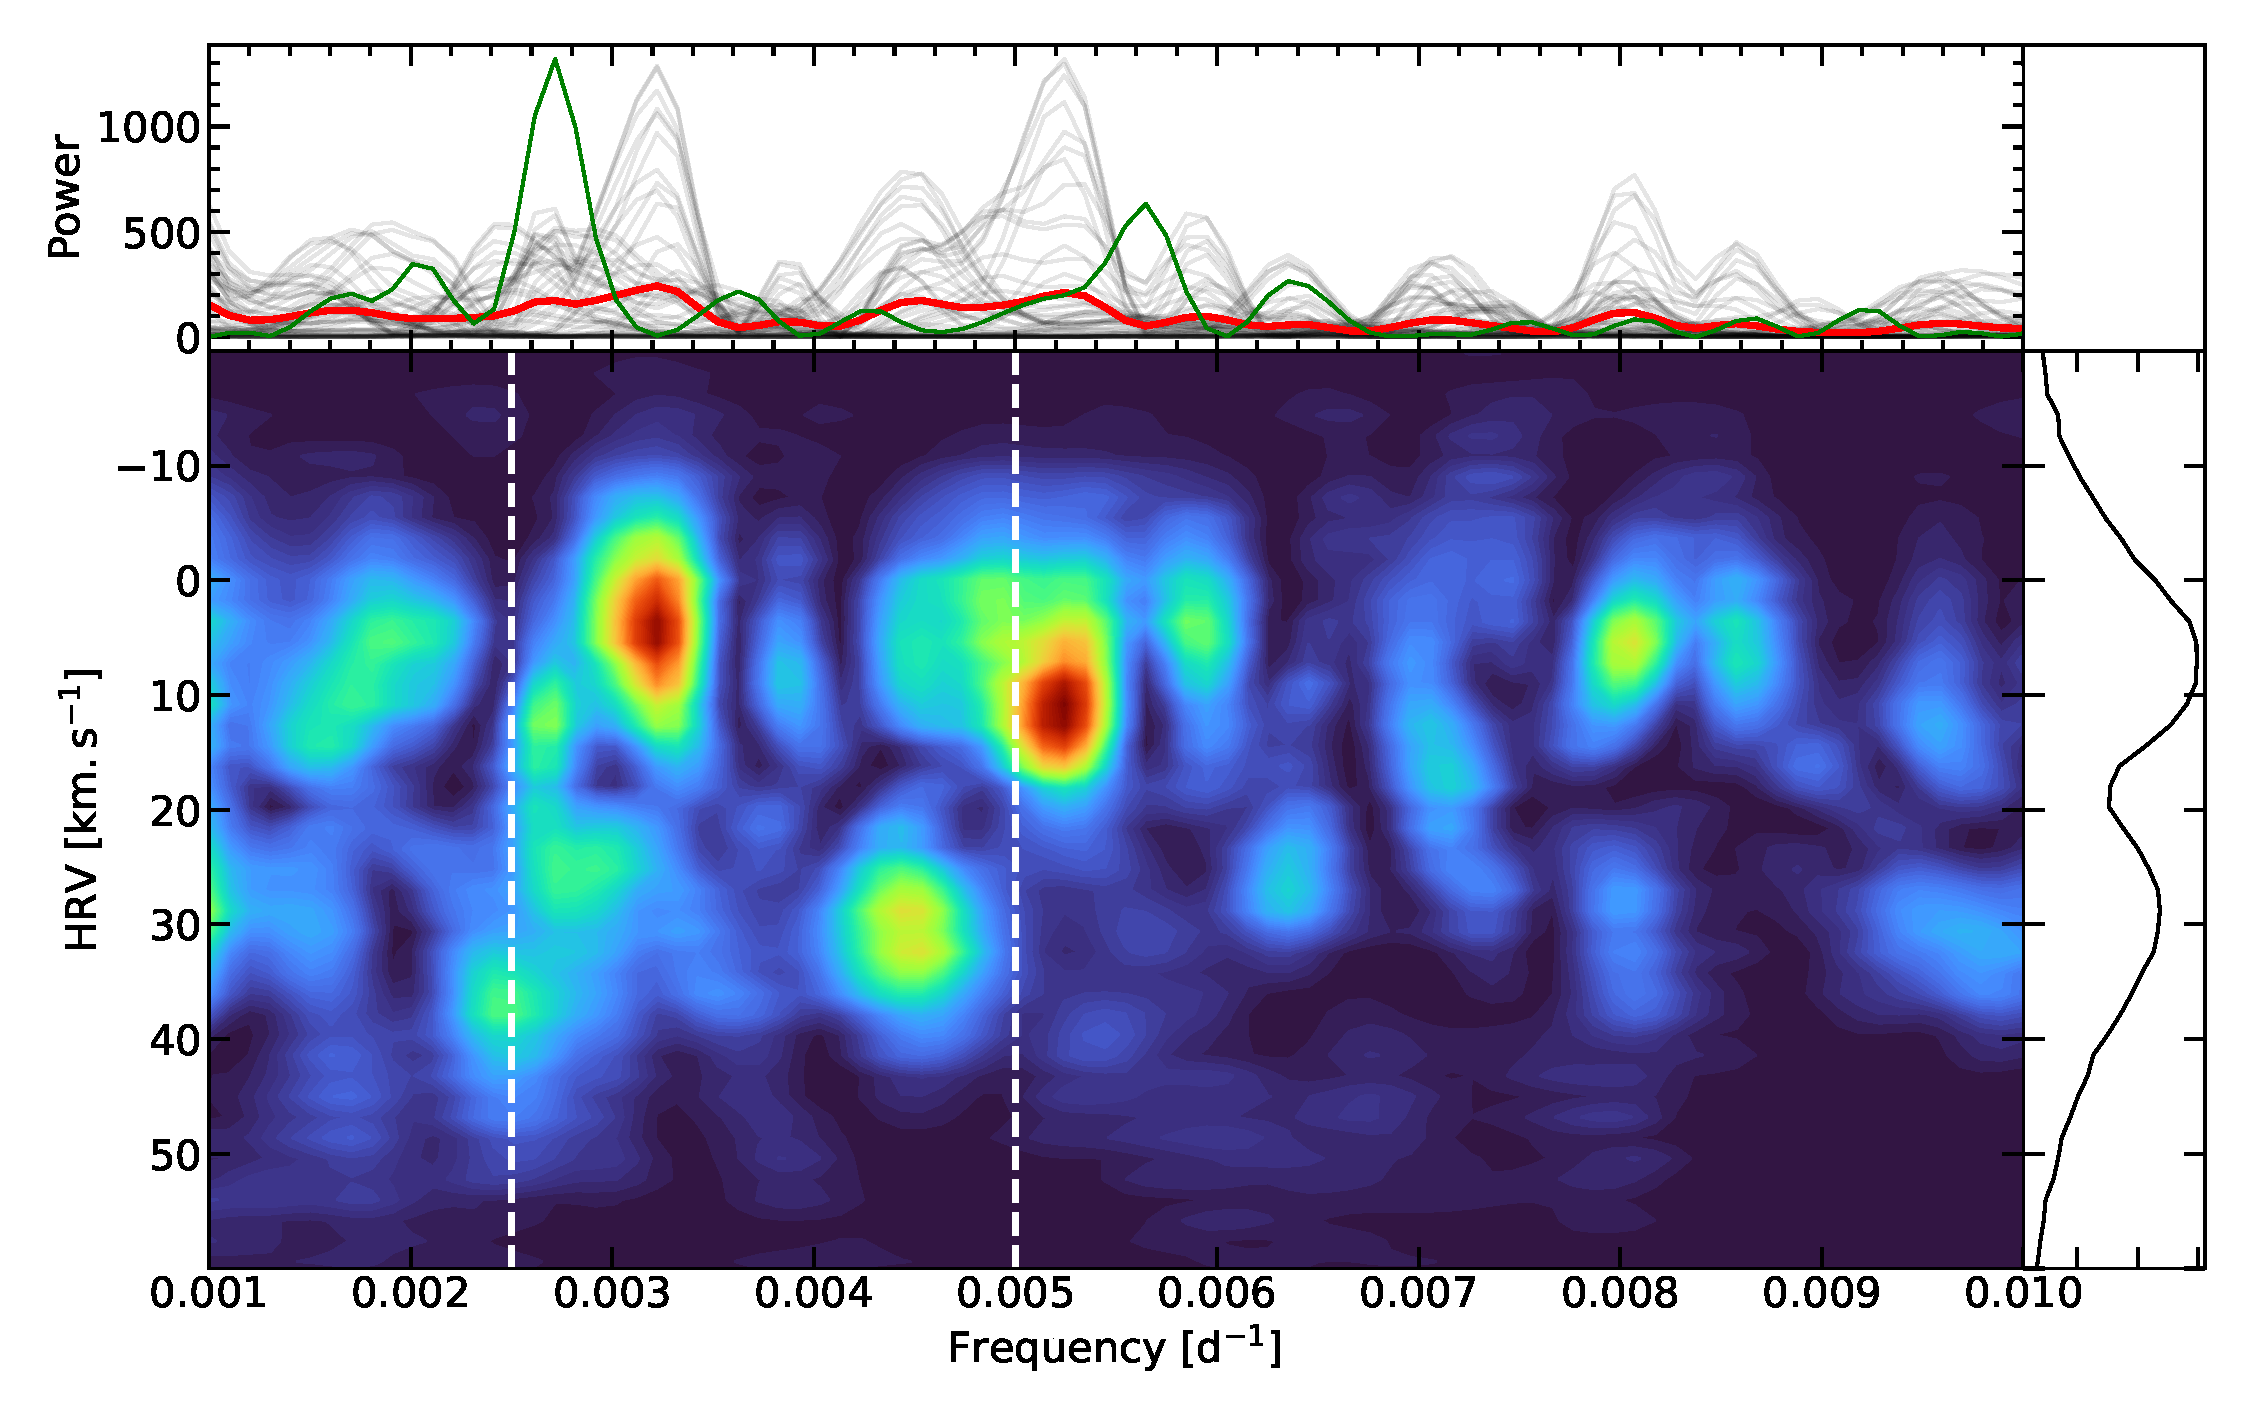
\includegraphics[width=0.5\textwidth]{Lomb-Scargle linear polarization.pdf}
    \caption{Same as Fig. \ref{LS intensity} for the total linear polarization: $\sqrt{Q^2+U^2}$.}
    \label{LS linear polarization}
\end{figure}



%\section{Recovering the variability of Betelgeuse in the LSD profile}

%\subsection{Intensity}
Examining Fig.\ref{LS intensity}, which shows the Lomb-Scargle periodogram of the LSD of the intensity profile, we observe that the 400 and 200 d periods seem to be captured by the periodogram. However, the 400 d period is uncomfortably close to the peak of the window function. Furthermore, both periods are located at the same HRV and in the blue wing of the profile. Interestingly, \cite{mathias_evolution_2018} previously found this 200 d periodicity in spectroscopic observation, despite of a shorter observation period. 



Figures \ref{LS Q} and \ref{LS U} display the Lomb-Scargle periodograms of Stokes $Q$ and $U$. These periodograms exhibit significant differences compared to the intensity one. In Fig. \ref{LS Q}, a prominent signal is evident around 200 d. Regarding Stokes $U$ in Fig. \ref{LS U}, it appears that the primary period is approximately $0.003 \ \mathrm{d^{-1}}$ (equivalent to 330 d). Other periods, such as those at 200 d or 250 d ($0.004 \ \mathrm{d^{-1}}$) are present, but are difficult to trust. From both periodograms of Stokes $Q$ and $U$, we recover the 200 d period, and also the 330 d period is notable, which aligns closely with the 400 d period reported in the literature and is in agreement with the timescale of the hysteresis loop reported by \cite{kravchenko_tomography_2019}.  
Figure \ref{LS linear polarization} shows the Lomb-Scargle periodogram of $\sqrt{Q^2+U^2}$, representing the total linear polarization of Betelgeuse. 
This periodogram confirms the significant powers at both 330 d and 200 d, consistent with the periodograms of Stokes $Q$ and $U$. 

%Nonetheless, the power of this period peaks at a HRV of around 40 km/s. We recall that this velocity is the rest velocity of the star. 
%Every signal beyond this velocity is either due to  plasma sinking in Betelgeuse, or to plumes of plasma rising beyond and above the limb of the star. 
%Such plumes from the back hemisphere have been often seen in other red supergiants like $\mu$ Cep \citep{lopez_ariste_height_2023}. 
%This suggests that both signals at these period of 400 days found in intensity and total linear polarisation 
%could well be due to the periodic appearance of plumes in the back hemisphere rising high enough to appear above
%the visible limb and generating a supplementary source of brightness. Once again we find a plausible explanation 
%of these periods unrelated to pulsations, but rather to the convective dynamics of the star.

% Up to this point, we want to pinpoint the two elements that are a clue 
% to understand the variability of Betelgeuse: the 400 days period is present in the linear polarization signal and also at a HRV above 40 km/s.
% In any case, from the linear polarization and the intensity profile, we recover the different periods of Betelgeuse. Since linear polarization is 
% associated to convection and because we recover the periods of Betelgeuse, the main mechanism behind the variability of Betelgeuse points toward surface convection.

\subsection{Variability of the polarimetric imaging}

Using linear polarization, \cite{lopez_ariste_convective_2018} successfully reconstructed images of Betelgeuse, which have been compared favourably to inteferometric images obtained by \cite{montarges_close_2016}. The images are produced by finding the brightness distribution that better fits the observed linear 
polarization LSD profile using a Marquardt-Levenberg minimisation.

Betelgeuse is observed, on average, every month by the TBL, enabling the tracking of its surface activity through this technique of polarimetric imaging. This technique has previously allowed for the estimation of  the size and the
 lifetime of convective cells on the surface \citep{lopez_ariste_convective_2018}. From these images, we computed a photo-center, a quantity sensitive to the size and number of convective cells. 
A homogeneous star will have a photo-center displacement coinciding with the barycenter of the star, whereas a star with one or two large convective cells will exhibit a more siginificant photo-center displacement, up to a few percent of the stellar radius in the case of RSGs \citep{chiavassa_probing_2022}. 

Since the photo-center is linked to surface convection, it is worth checking for periods in its 
dynamics over the 5 years of observations of Betelgeuse before the dimming. While these periods may overlap with those presented in the previous section, they are likely to capture additional aspects of the phenomena at work.

%We computed the Lomb-Scargle periodogram of the displacement of the photo-center.
However, before proceeding to search for periods in the displacement of the photo-center, it is important to address a key issue regarding the interpretation of such images. 
Linear polarization suffers from a $180 ^\circ$ degree ambiguity, as mentioned in \cite{auriere_discovery_2016}. Consequently, our images 
can be 
rotated by $180^\circ$ degrees, and the brightness distribution will still fit the observed LSD polarization profiles. 
If each observation were treated independently, the algorithm's solution could be any of the possible ambiguous solutions. To ensure continuity 
between the image series, 
for a given day, we use the brightness distribution of the previous day as the initial point 
of the  fitting iteration. The first image in the series begins its minimisation iteration with a random brightness distribution. 
Although we can produce a series of consistent images, it is important to keep in mind that the photo-center displacement computed from the series 
will be affected by the initial image. 
To overcome this issue, we computed
the photo-center displacement from 100 different time series, each starting from a different initial image. This approach aims to recover ensemble properties independent of the choice of the first image. 

\begin{figure}[!h]
    \centering
    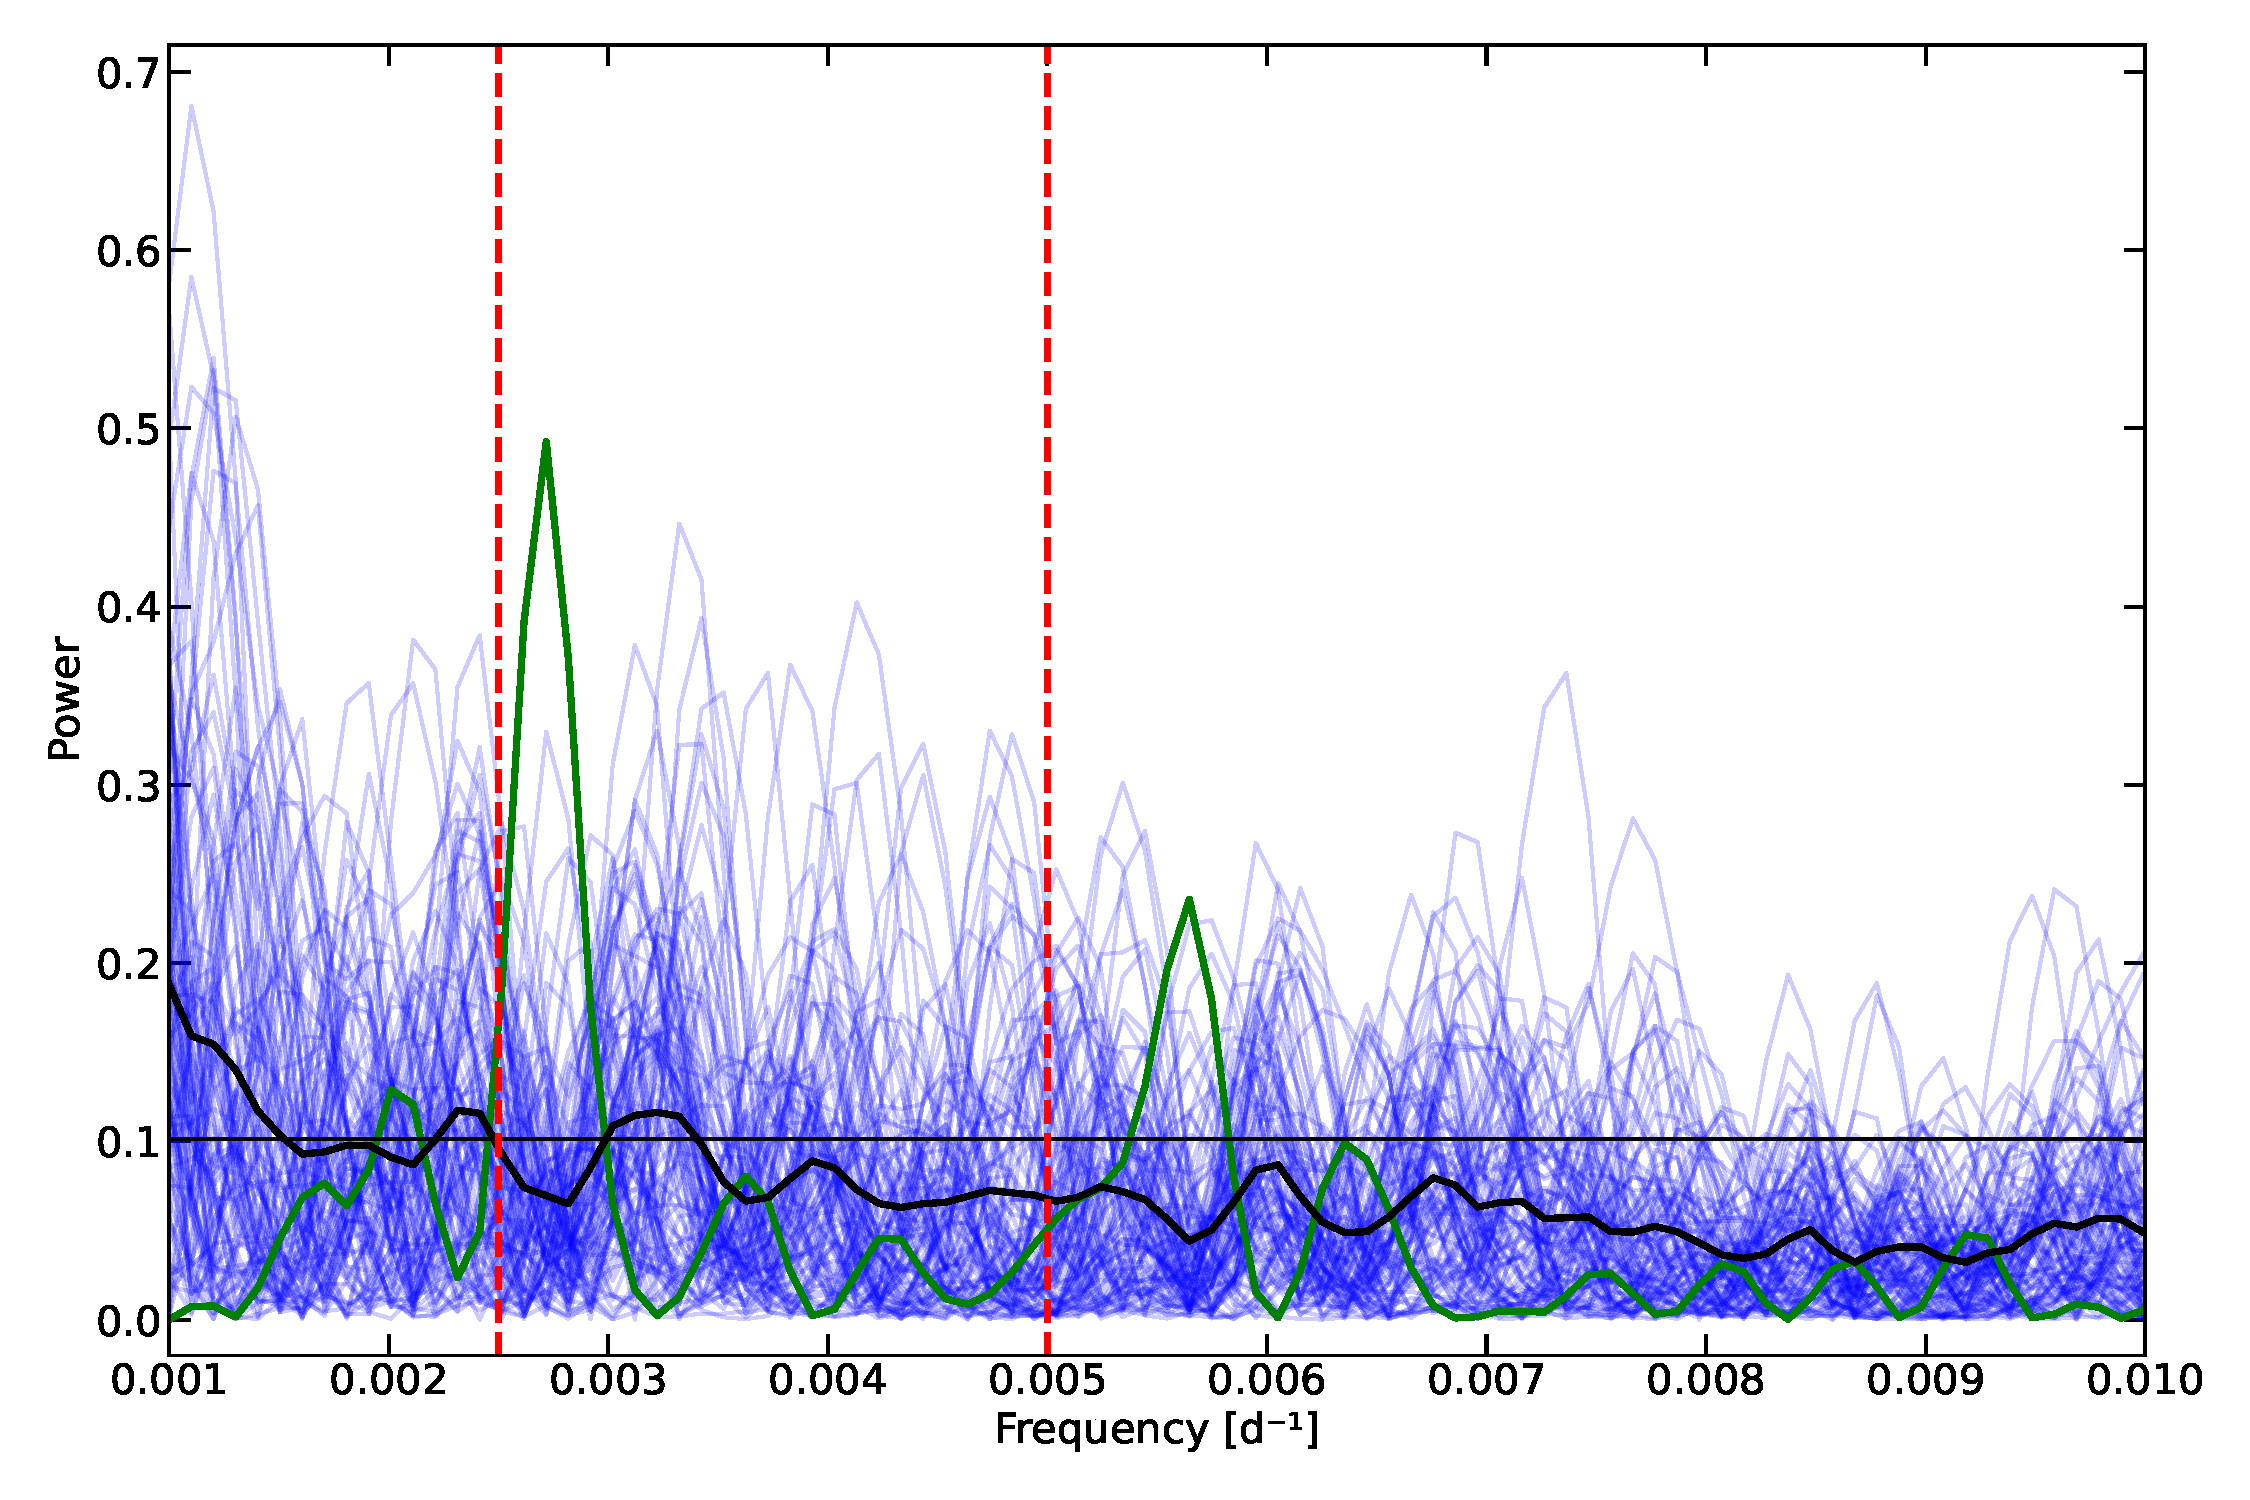
\includegraphics[width=0.5\textwidth]{Lomb-Scargle Photo-center.pdf}
    \caption{Lomb-Scargle periodogram of the 100 photo-center displacement series of Betelgeuse. Each blue line corresponds to a Lomb-Scargle periodogram of one photo-center
     displacement. The black line is the average of the 100 periodograms. The red dashed lines represent the 400 and 200 d period respectively. The green line is the window function.}
    \label{LS photocenter}
\end{figure}

Figure \ref{LS photocenter} shows the Lomb-Scargle periodogram of the photo-center displacement for each of the 100 series (blue lines) and the average Lomb-Scargle periodogram (black line). 
%As before, the upper panel shows the Lomb-Scargle periodogram from data before the great dimming only, whereas we used the whole set of data for the lower panel.
The red dashed lines indicate the 400 and 
200 d periods, respectively. Similar to previous figures, the window function is represented by the green line. Interestingly, we find two peaks around the 400 d period in the periodogram, although they are not individually significant to confirm the presence of such period. However, these peaks are consistent with the findings of the previous section. Since polarimetry imaging involves only surface convection, this provides further support for a variability being explained by surface convection alone.


\subsection{Variability of the light curve}

After examining the periods identified by the Lomb-Scargle technique in the polarization data obtained by the TBL over the last years before the dimming, it is worth contextualizing them alongside the periods traditionally identified in light curves over the same period of time. Two aspects 
are of our interest in this comparison: the behaviour of the light curve before and after the great dimming.

\begin{figure}[!h]
    \centering
    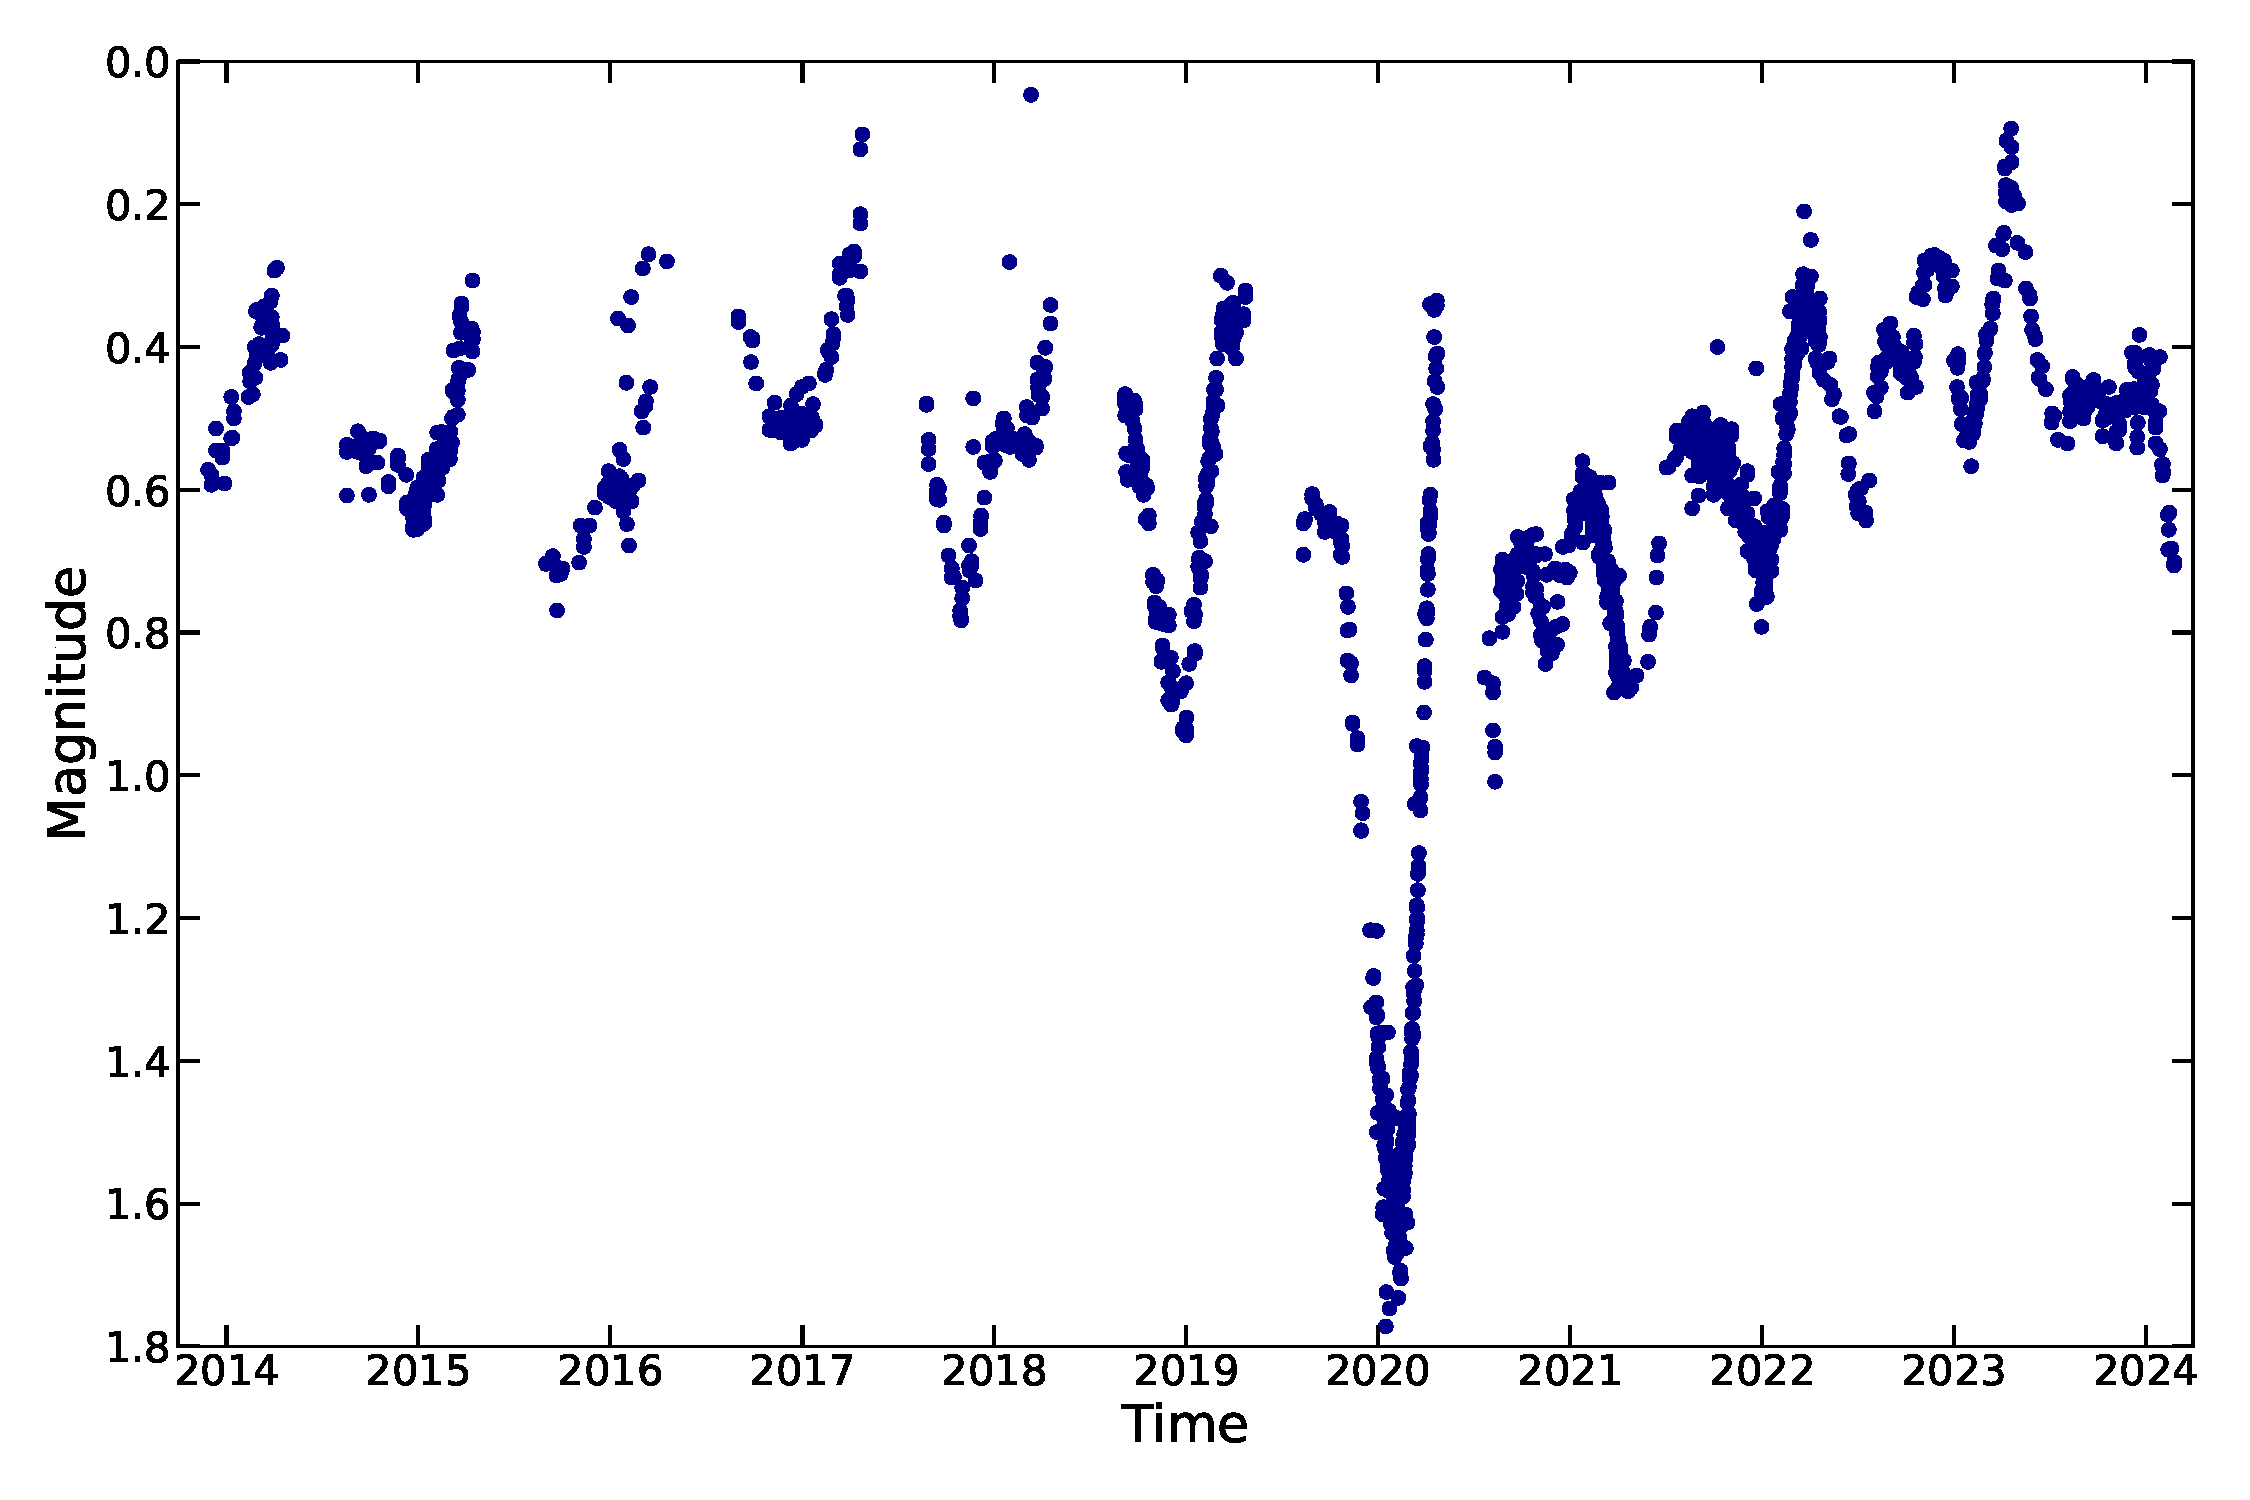
\includegraphics[width=0.5\textwidth]{Light_curve_Betelgeuse.pdf}
    \caption{Light curve of Betelgeuse from AAVSO in the V-band.}
    \label{light curve Betelgeuse}
\end{figure}


We have retrieved the light curve of Betelgeuse in the visible from the AAVSO database for the past 10 years. It is shown in Fig. \ref{light curve Betelgeuse}.
Before the great dimming, Betelgeuse's magnitude exhibited variations on a yearly timescale, whereas after the dimming, its variability has shortened. 
Figure \ref{light curve Betelgeuse} clearly illustrates that the 
variability of Betelgeuse now occurs on a timescale shorter than one year. This qualitative change has been pointed out before,
before the great dimming, the primary period of Betelgeuse was approximately 400 d \citep{kiss_variability_2006}, often associated with the fundamental pressure mode. However, after the dimming, this period seems to have vanished, and only timescales shorter than 230 d are visible since \citep{dupree_great_2022}. 
No explanations have been put forth regarding this change of variability after, or perhaps because of the dimming.% In  Section \ref{section 4},  we  afford proposing alternative scenarios for the observed periodicities in the light curve.\\

 In Fig.\ref{Lomb Scargle AAVSO}, we computed the periodogram from that light curve of Betelgeuse (blue line), alongside the periodogram computed exclusively with AAVSO observations made less than 2 days from our observation dates of the TBL (orange line). 
 For the periodogram since 1990, we binned the observations with an interval of 10 days, as Betelgeuse has been more observed in the 21st century \citep{kiss_variability_2006}. This periodogram  recovers the 400 d period and also a period close to 200 d. Other visible peaks are rather 
 due to the windowing effect.   However, when focusing on the periodogram derived from the light curve corresponding to the TBL observation dates, we fail to retrieve the periods mentioned in the literature. The periodicities found in the TBL observations 
 gain validity through this comparison: they were evident in the TBL data, but barely recovered in the AAVSO data when pruned to the same observing dates. We can anticipated that extended spectropolarimetric observations 
 of Betelgeuse will make these periodicities seen in linear polarization, and arising from convective structures, clearer and clearer.


\begin{figure}[!h]
    \centering
    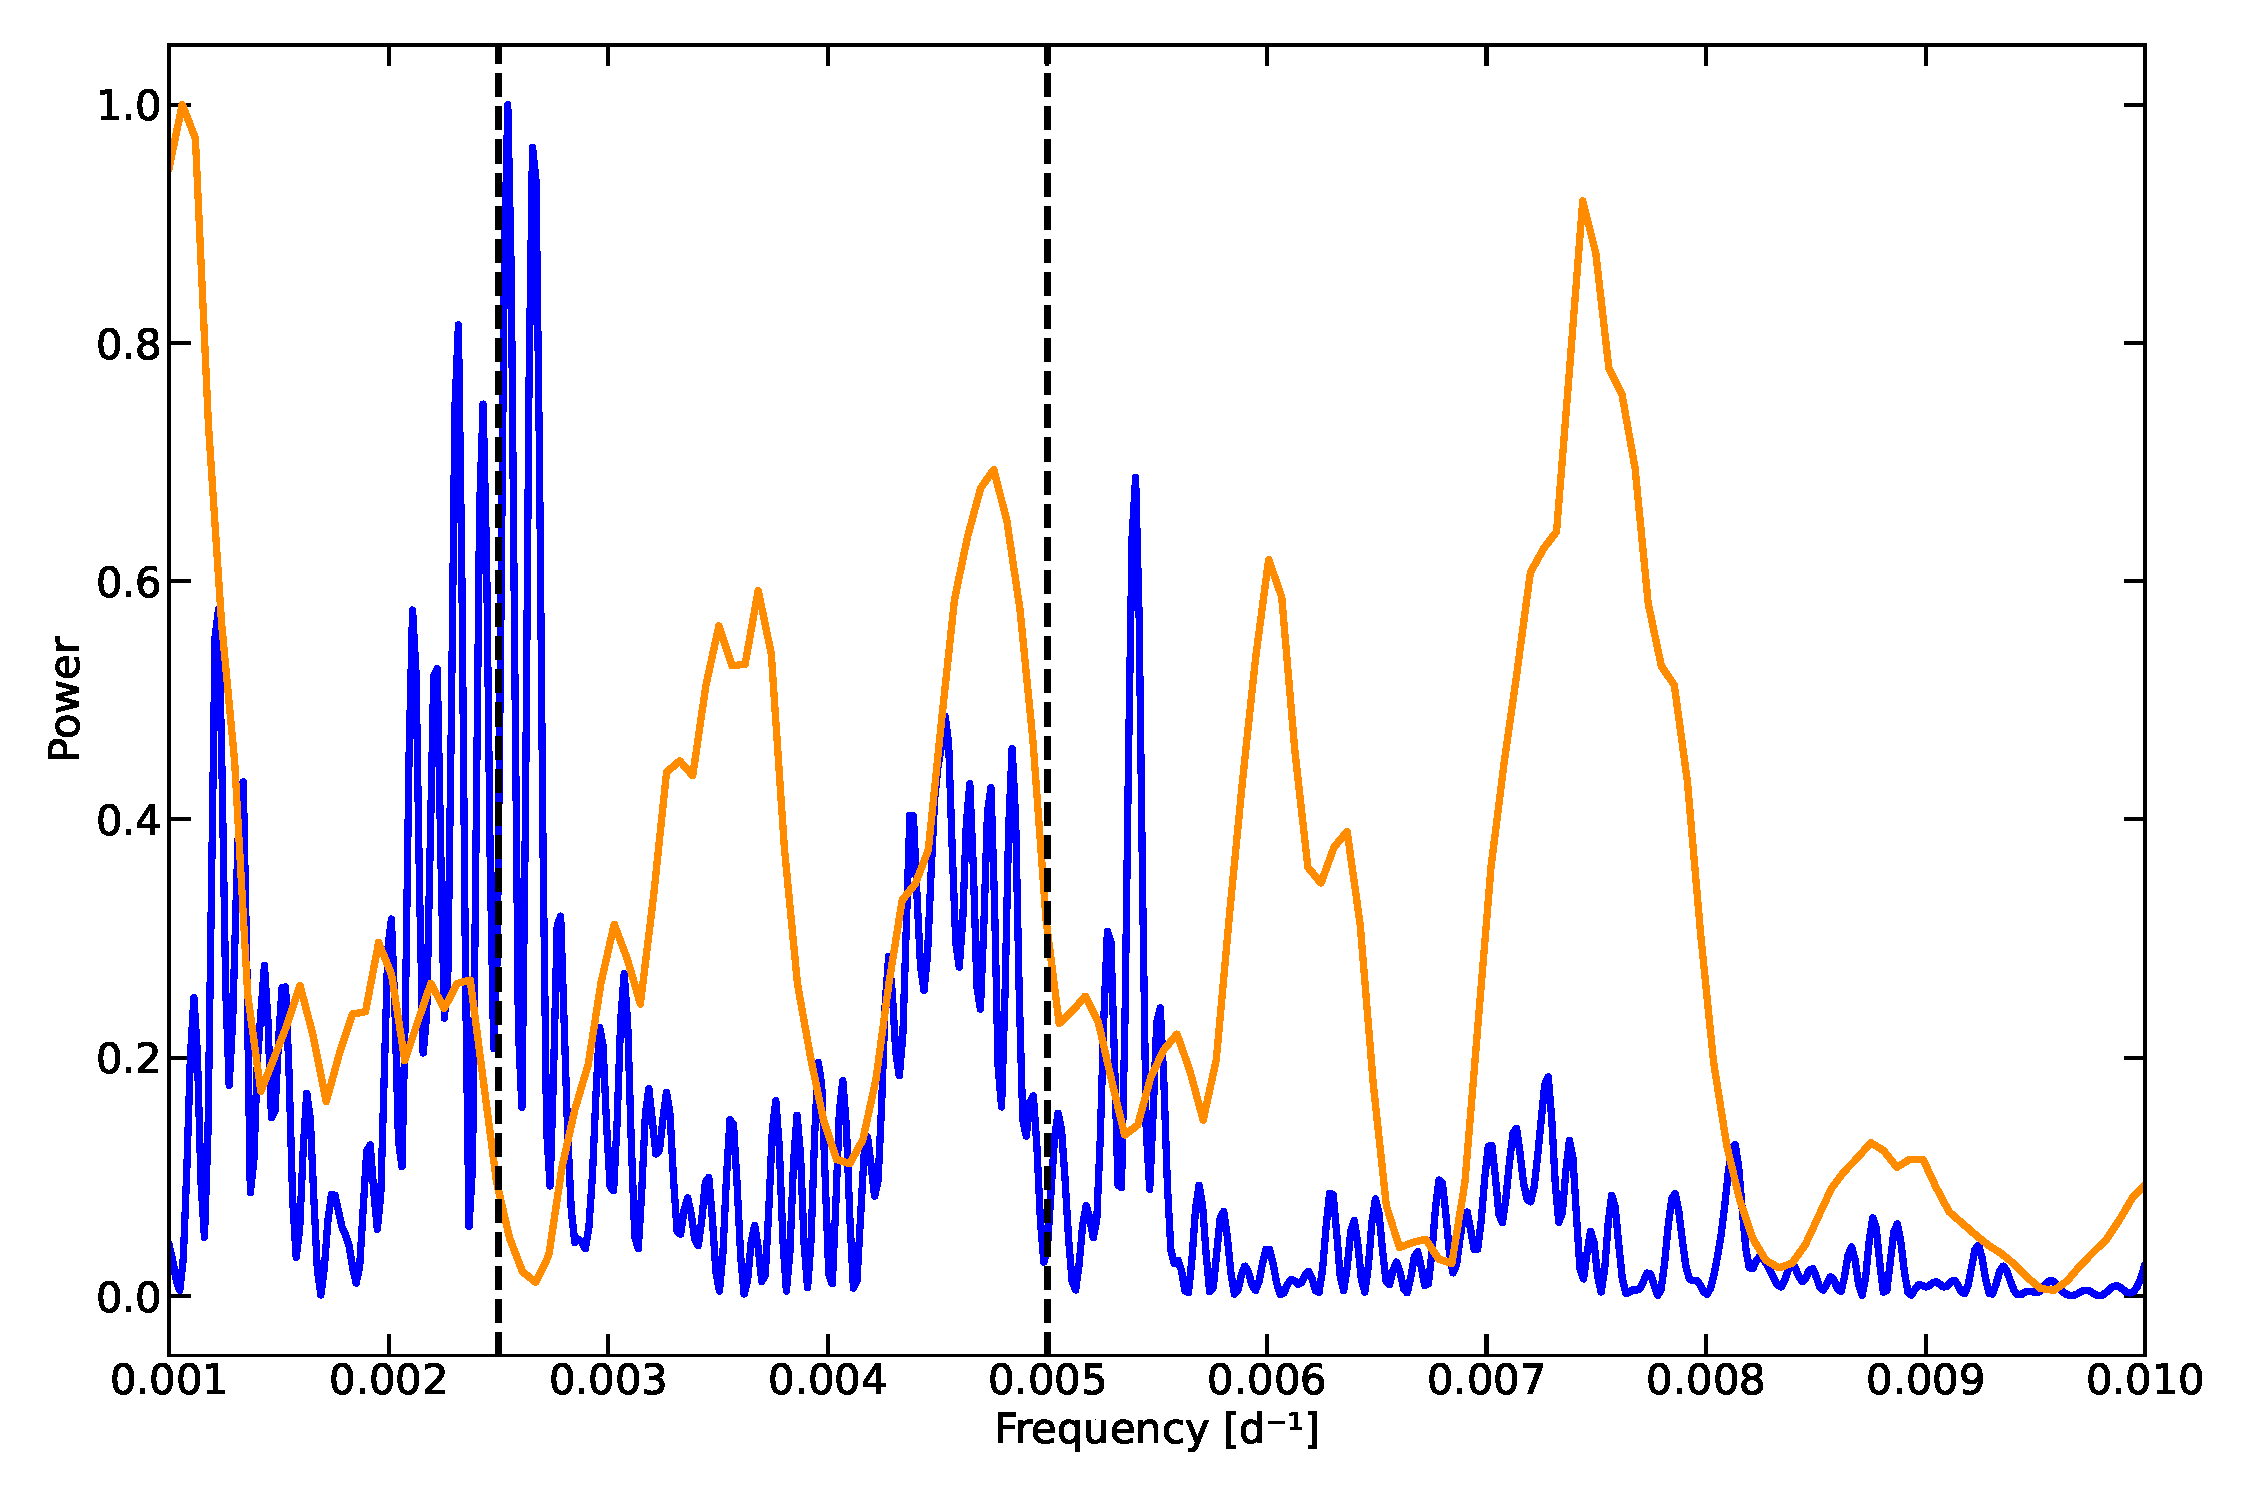
\includegraphics[width=0.5\textwidth]{Lomb-Scargle AAVSO.pdf}
    \caption{Lomb-Scargle periodogram of the light curve of Betelgeuse since 1990 as retrieved from the AAVSO database (blue line). When only dates corresponding to TBL observations are retained in 
    that light curve, the periodogram in orange color is obtaine. The two black dashed lines are respectively the 400 and 200 d periods for visual reference.}
    \label{Lomb Scargle AAVSO}
\end{figure}

\section{Discussion}
\label{section 4}
%Before summing up the conclusions of this work, we can afford proposing alternative scenarios for the observed periodicities in the light curve, 
%the LSD profiles and the displacement of the photo-center of the inferred photospheric image reconstructions. 
The presence of the same 
periods and, considering the time span and sparsity of the TBL data series, the larger amplitude of the peaks found in
polarization data when compared to those in the light curve point to a common origin in either observation, one that is rather based upon convective dynamics. Since we associate Stokes $Q$ and $U$ to proxies of convection, we associate the 200 d period to the typical timescales on which the Stokes parameters evolve. 
The LSD profiles of Stokes $Q$ or $U$ undergo slight changes when observing Betelgeuse monthly, but are completely overhauled 
on time scales of several months. The Lomb-Scargle periodograms seem to capture this spectral dynamic at periods of aproximately 200 d. Such changes in the profiles are directly linked to the dynamics of the surface,  to  the evolution, and movements 
of convective cells across the visible hemisphere. Therefore, the 200 d period appears to be related to the evolution of the convective patterns 
on the surface of Betelgeuse.  The stronger presence of this peak in Stokes $Q$ compared to $U$ could be interpreted as a temporal situation of how convective patterns have been distributed in the
last years.\

The other period found in the total linear polarization and Stokes $U$, the 330 d periods, is not so far from the 400 days period often mentioned in the literature (e.g \cite{kiss_variability_2006} found a period of $388 \pm 30$ d). It has been shown by \cite{lopez_ariste_convective_2018} that large convective cells can persist for one to two years. Thus, the 330 d period could be associated to the timescale on which the largest granules evolve. This characteristic timescale has also been observed in the numerical simulations and might play an important role in determining stellar distances through the displacement of the photo-center \citep{chiavassa_probing_2022}. Once again, we observe the 330 d periodicity to be more prominent in Stokes $U$ than in $Q$, what may unravel a random situation due to convective motions in the last years. This interpretation aligns with the work of \cite{gray_mass_2008}, who attributed the 400 d period to 
large convective cells. Whether this 330 d period and the commonly cited 400 d period are one and the same will have to wait for extended spectropolarimetric observations with the TBL that smooth the windowing function around these frequencies.

Regarding the Stokes $I$ profile, a peak closer to the 400 d period appears, but it is once again uncomfortably close 
to a peak of the window function of the TBL, making it difficult to trust. A secondary peak close to 200 d is also present in the Stokes $I$ profile, that we fully assimilate to the one found in the Stokes parameters, and that  we attribute to convective timescales. 
%Up to this point, the model developed to interpret linear polarization involves only surface convection, which is why we interpret the 200 d period as the convective timescale of the smallest structures, while the 400 d period corresponds to the timescale of the largest structures.\\
 %As showed by
%\cite{lopez_ariste_convective_2018}, some of those convective cells can live up for years. We may speculate
%that the LSP may be related to those long living structures. However the present span of data from the TBL is insufficient to do more than
%just speculate. It should be noticed that  
% the peak is not present in stokes U, and this may point to a more stochastic event than just long-living structures.



Before summing up the results of our work, we can afford to propose an explanation for the variability of Betelgeuse after the great dimming with surface convection. RSGs experience mass loss events when plasma is ejected into the interstellar medium \citep{josselin_atmospheric_2007}. 
These events have been inferred in RSG such as $\mu$~Cep at photospheric heights, where \cite{lopez_ariste_height_2023} found an excess of linear polarization beyond the limb of the star, attributing it to rising plumes of plasma in the back hemisphere of the star. 
In the case of Betelgeuse, the excess of linear polarization beyond the limb is rare and not as pronounced as those observed in $\mu$~Cep. They do not appear to contribute to 
 the variability of the star. However, since the great dimming, the variability of Betelgeuse has changed. This suggests that the great dimming differed significantly from the usual mass loss event, and perhaps it hustled the  photosphere. \

In a scenario where the variability of Betelgeuse is primarily governed by convection,  the visible periods of such variability  were associated, before the great dimming, to the 
typical timescales at which convection occurs: approximately 200 d for the small structures and roughly 350 d for the large structures. The great dimming affected the behaviour of the photosphere in such a way that the largest structures 
no longer evolved on a timescale around 350 d, but rather on the shorter timescales of the smallest convective structures, around 200 d. We hypothesise that after the great dimming event, the photosphere has not yet returned to equilibrium, and the largest convective structures 
have been disrupted by the turbulent motions present of the photosphere in this period. This would explain why identifying the longer periods after the great dimming has been hard, as \cite{dupree_great_2022} noticed. We may expect that the 400 d 
period will gradually reappear in the coming years as the photosphere returns to equilibrium. However speculative, this scenario 
provides a rough explanation of how convective activity could lead to a change in variability since the great dimming that future observations and 
research will confirm or infirm.
%A more detailed explanation of this variability change falls beyond the scope of this paper and is left for future research.
%But this 
%is a behaviour that fully concurs with what we find in the polarization data, and which cannot be related to any stellar pulsation but rather 
%convective dynamics. Beyond the actual values of the periods found in a Lomb-Scargle periodogram, we also see a correspondence between polarization 
%and the light curve in these changes in the observed periods before and after the great dimming. Such concurrence points to an explanation 
%in terms of convective dynamics also for the variability of the light curve.


%It may be argued that the periodograms presented in the previous sections and, in particular, those  of the photo-center displacements, 
%present low amplitude peaks at the referred main periods. One may wonder whether we are over-interpreting mere fluctuations of the periodograms, 
%while the peaks seen in the literature from analysis of the light curve are unmistakable. It is therefore worth to take advantage of the 
%availability of the AAVSO data to perform a Lomb-Scargle periodogram of the light curve in the same period covered by our polarization data and,
%furthermore, taking into consideration data around the dates for which TBL data is available. Periodograms  with such constraints are 
%shown in Fig.\ref{LSAAVSO}. Even when the full dataset for the period is taken into account (red line), the periods present small amplitudes, and are 
%fully and favourably comparable with the periodograms presented above. This is even more dramatic when the periodogram is made from data at the exclusive 
%dates at which TBL data is available (blue line). It stands out that the low amplitude peaks are rather due to both the sparse cadence and short span of 
%time of the TBL data series rather than to a physical absence. Actually, the present tests puts more emphasis on the importance of the 
%strong peaks seen at selected wavelengths in the LSD profiles, strong when compared to the peaks at similar periods arising from the light curve. 



%\begin{figure}[!h]
%    \centering
%    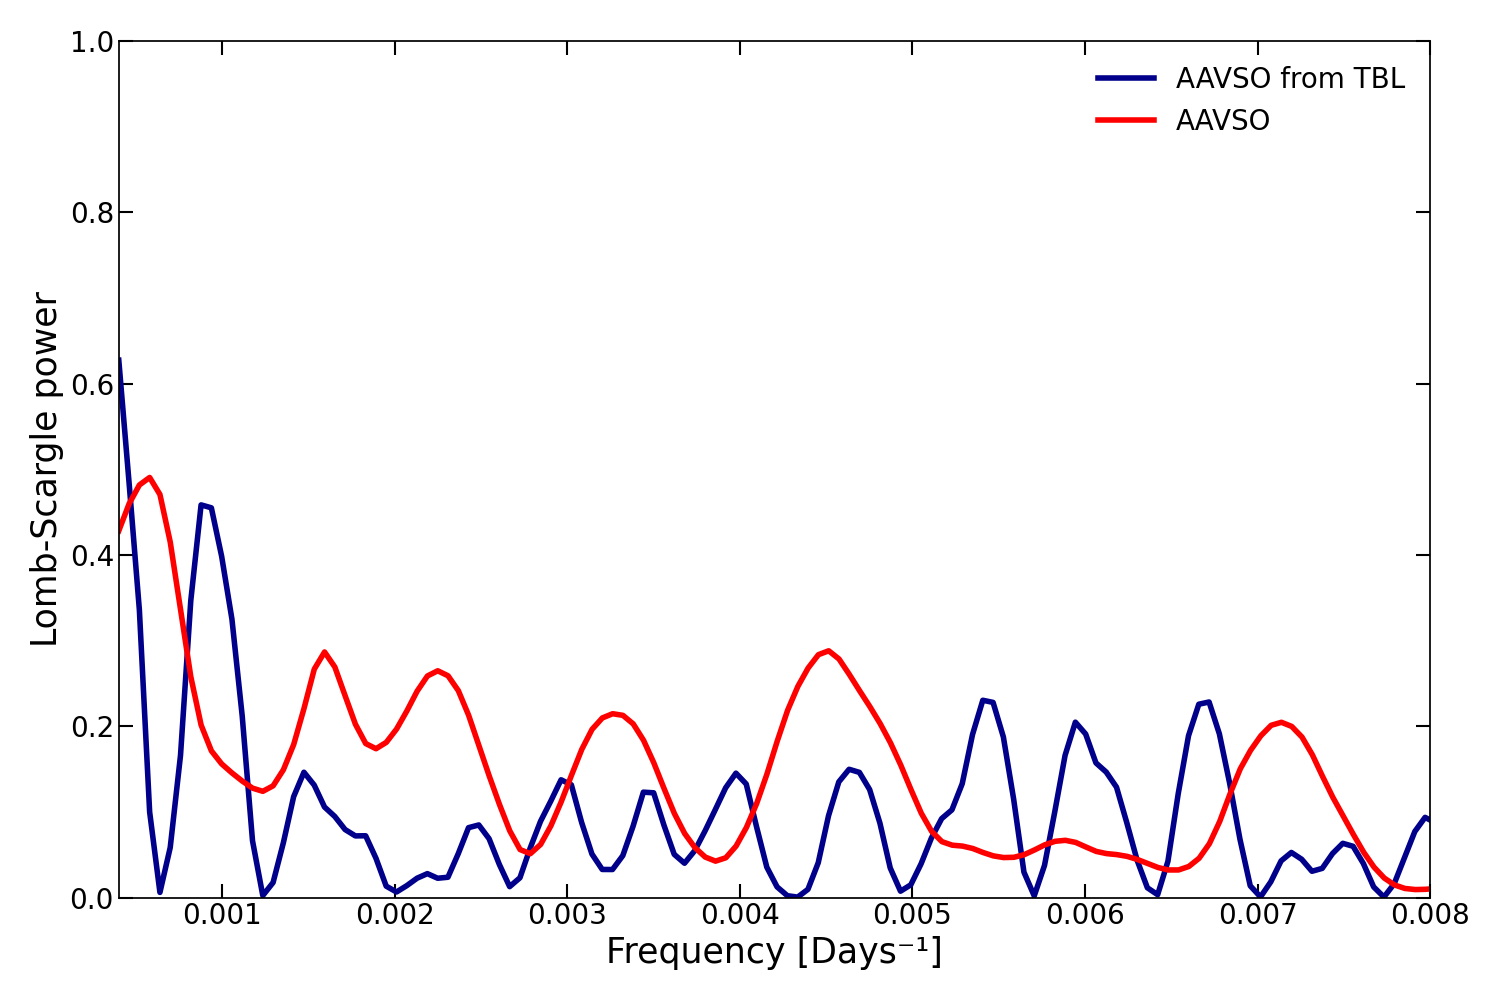
\includegraphics[width=\linewidth]{Lomb-Scargle-TBL.png}
%    \caption{Lomb-Scargle periodogram from the AAVSO data between 2013 and 2023 (red line) and from the AAVSO data taken near TBL observations (blue line).}
%    \label{LSAAVSO}
%\end{figure}

% constant, which is not consistent with a pulsating scenario. The constant magnitude of Betelgeuse points toward another scenario than pulsation. Using surface 
% convection, we can fully explain the variability of Betelgeuse. The oscillations in the light curve are due to two mechanisms: surface convection and rising 
% plumes of plasma beyond the limb of the star. This last mechanism being random, it happens from time to time. The timescale on which convective cells evolve
% is between one and two years, which is also consistent with the 400 days period found in the literature.  After the dimming, the change of periodicity in the
% light curve is explained by surface convection, the random variation of brightness distribution could lead to the 200 days periodicity found in the literature. 
% The constant brightness of Betelgeuse for the last 6 months is explainable by the same random brightness distribution: the surface of Betelgeuse is calm, 
% leading to this constant brightness. In the future, we expect to see the light curve of Betelgeuse to change, maybe with another main period, but which 
% is in fact caused by surface convection. Thus, the main mechanism in the variability of Betelgeuse is surface convection, which is sufficient to explain the 
% variation in the magnitude of Betelgeuse.  






%and not to radial or 
%other global pulsations.

% We recall that while the nature of the LSP is still in debate, the nature of the lower periods is quite commonly 
% attributed to  pressure modes 
% (e.g \cite{kiss_variability_2006}). The mechanism behind the pulsation of Betelgeuse is attributed to the $\kappa$-mechanism. In this 
% section, we attempt to 
% find an explanation to the 400 days periodicity of Betelgeuse. 
% As mentioned before, the LS periodogram of linear polarization shows a periodicity 
% around 400 days. Furthermore, the region where the LS power is high is around 40km/s. 
% This wavelength corresponds to most redshifted signal present in Betelgeuse.

%The 400-day period appears prominently in both the intensity and the total polarization profiles. And in both cases, it is mostly present 
%at wavelengths in the red wing, often beyond the 40 km/s value.
%We recall that in the present scenario for the formation of the polarization signal, this signal is supposed to remain between 
%-20 and +40km/s. Signals above 40km/s are uncommon and can be associated to
 %plasma rising behind the limb of Betelgeuse. 
%Such scenario has been observed in the RSG $\mu$ Cep and was introduced by \cite{lopez_ariste_height_2023} to explain the excess of 
%linear polarization beyond  the rest velocity of the star, which for Betelgeuse is fixed at +40km/s. 
%In $\mu$ Cep, such  linear polarization signal beyond the limit of the rest velocity of the star is very strong and particularly 
%common, two features that prompted a dedicated explanation. In Betelgeuse, such signals, when present, are weaker. However, 
%they are visible from time to time, with regularities that are captured by  the Lomb-Scargle periodogram at 400 days.
%Without further justification, we may propose that convective plumes in the hidden hemisphere of the star and 
%rising above the limb from time to time are responsible for the  400 days period in the light curve. When such plumes rise high enough 
%to be geometrically visible above the limb they show signals in intensity and polarization at redshifted wavelengths. They also
 %increase the emitting surface of the star and  the number of photons that we receive,
%leading to an increase of the brightness visible in the light curve. After a few weeks or months, the plume falls back to Betelgeuse, 
%disappearing from our point of view,  leading to a decrease of the brightness.

%The appearance of such high-rising plumes is not necessarily periodic. And the star can easily shift from active periods when such 
%plumes are a common feature to calmer periods when no plume is visible for months. $\mu$ Cep may be in one such active period presently,
%while Betelgeuse may have experienced recently one great such event in the direction of the Earth that, after dust formed, became the great 
%dimming, but since then no other high-rising plume has appeared, explaining the absence of the 400-day period since the great dimming. 
%From the point of view of convective dynamics we can offer an explanation of the 400-day period which not only explains the observation of 
%this period both in the light curve and in the polarization profiles, but also its presence at redshifted wavelengths and its present (and probably 
%temporary) disappearance since the great dimming.


% This is exactly what we see in the LSD profile of the linear polarization of Betelgeuse: 
% from time to time, there is a net signal above 40km/s, which is present for a few weeks, and then disappears. Since this signal is not always present, 
% it is found by the LS periodogram as a periodic event. However, it is not periodic at all: because the plumes rise at random moments, sometimes they 
% appear every years, sometime they do not. This would explain why we only see it before the dimming. After the dimming, this kind of event never happened 
% for the moment. Thus, the LS periodogram, at that precise frequency, finds that there is a periodic signal before the dimming, but not after, leading to
% a lower LS power at this frequency.



% To summarise what we have done so far: we were able to explain the variability of Betelgeuse using surface convection only. The convective cells play 
% the most important role in the variability of Betelgeuse. Our work does not need pulsation to explain its variability. This does not mean that there are 
% no pulsation in Betelgeuse. What we claim is that the most important factor in the variability of Betelgeuse is the timescale on which the convective 
% cells evolve. Pulsation could exist on Betelgeuse, but they are not the main contributor to the variability. 




\section{Conclusion}
\label{Conclusion}

The main result presented in this work is that the same periods identified in the light curve of Betelgeuse are also observed in the intensity and polarization
spectra measured with the TBL. Traditionally, periods in the light curve have been associated to pulsations due to pressure modes.
%But such pulsation would in no case affect the polarisation signals nor would explain the fact that the periods can be observed with stronger 
%amplitude at selected wavelengths but no others. % Pulsation appears to offer no coherent explanation to these observations, are hardly to the 
%observed changes in the variability since the great dimming.  The concurrence of observational facts, actual period values, evolution before 
%and after the dimming, the larger amplitude of the period peaks in polarizarion data, points towards a common origin for those variabilities. 
%And such origin cannot be pulsations.
However, the interpretation of the linear polarization profiles is made in terms of convective structures in the atmosphere of Betelgeuse. We propose that the true reason for the observed periodicities in both the light curve and spectropolarimetric observations lies within these convective structures and their temporal evolution.
This is the main conclusion of our work: since we are able to recover the different periods in the linear polarization profiles, we can exclude pulsation phenomena as the explanation for those periodicities in the light curve. This conclusion concurs with the scenario proposed by \cite{gray_mass_2008}, attributing the variability of Betelgeuse to surface convection.
 We further find hints in the polarized spectra that lead us to associate the 200 d periodicity to convective dynamics, while the 400 d periodicity may be linked to convective timescales of the largest granules.  
%the observed periods are related 
%to convective dynamics and not to radial pulsations of the star.

Although of secondary importance, we can speculate on the phenomena underlying the change in variability before and after the great dimming event. We hypothesize that the great dimming event disrupted the dynamics of the photosphere, 
leading to the destruction of the largest granules by the turbulent motions present in the non-equilibrium of the photosphere after such event. Since this happened, the variability of Betelgeuse has quickened in adequacy with the timescale of smaller convective cells, around 200 d. If this scenario is correct, we shall expect in the coming future, the re-emergence of the 400 d variability as the dominant period once the photosphere returns to some form of equilibrium. Longer time 
series of spectropolarimetric observations of Betelgeuse will be necessary to provide further insights into this phenomenon.

%Although of secondary importance, we may suggest with more or less ease what phenomena are at the origin of the main periods. The 400-day period 
%appears to be strongly related to the appearance of plumes in the back hemisphere of the star rising high enough to be seen above the limb.
%Such plumes have been described in another RSG, $\mu$ Cep, and while less common or prominent, they are also present in Betelgeuse. The irregularity 
%of their presence justifies the 400-day period, which is captured by the Lomb-Scargle periodogram in the polarization signals attributed to 
%this phenomenon. The redshifted wavelengths at which this periodicity is found are justified by the plume moving away of the star and of the Earth while 
%raising in the back hemisphere, while the brightness increase is justified by %the extra surface of emitting plasma visible. The 200-day period is less 
%prominent but appears to be correlated to the typical time scales of the evolution of the convective structures themselves on the visible hemisphere. 
%The LSP origin is harder to pinpoint given the insufficient time length of our time series. One can speculate if it may be related to the 
%longest living photospheric structures, but this explanation does not adequately explain all the features associated to this period. Longer time 
%series of spectropolarimetric observations of Betelgeuse will be required to shed light on this.




\begin{acknowledgements}
    This work was supported by the "Programme National de Physique Stellaire" (PNPS) of CNRS/INSU co-funded by CEA and CNES.
    We acknowledge support from the French National Research Agency (ANR)
    funded project PEPPER (ANR-20-CE31-0002).
    We acknowledge the observers of the AAVSO International Database who provided more data than enough to produce this work.
    
    \end{acknowledgements}
    
    \bibliographystyle{aa}
    %\bibliographystyle{aa}
    
    \bibliography{art75}
\end{document}
